

\documentclass[11pt]{article}
\usepackage[utf8]{inputenc}
\usepackage{geometry}
\usepackage{graphicx}
\usepackage{hyperref}
\usepackage{amsmath}
\usepackage{listings}
\usepackage{xcolor}
\usepackage{float}
\usepackage{subcaption}
\usepackage{algorithm}
\usepackage{algpseudocode}
\usepackage{booktabs} % For prettier tables
\usepackage{siunitx}
\usepackage{amssymb}
\usepackage{subcaption}

% Set page margins
\geometry{a4paper, margin=1in}

% Set up code listing style
\lstset{
    basicstyle=\ttfamily,
    commentstyle=\color{gray},
    keywordstyle=\color{blue},
    stringstyle=\color{red},
    showstringspaces=false,
    captionpos=b
}

\title{Diffusion models: M2 coursework report}
\author{Vishal Jain}
\date{\today}

\begin{document}

\maketitle

\tableofcontents
Word count: 2934 (not including appendix)
\newpage
\section{Background}
\subsection{Latent Variable Models}
Latent variable models are probabilistic models that model the probability distribution of the data $Pr(\mathbf{x})$ through the use latent variables $\mathbf{z}$. They define a joint distribution $Pr(\mathbf{x}, \mathbf{z})$ of the data $\mathbf{x}$ and an unobserved hidden / latent variable $\mathbf{z}$. They then describe $Pr(\mathbf{x})$ as a marginalisation of this joint probability over the latent variables:

$$
Pr(\mathbf{x}) = \int Pr(\mathbf{x}, \mathbf{z})dz.
$$

$$
Pr(\mathbf{x}) = \int Pr(\mathbf{x}|\mathbf{z}) Pr(\mathbf{z})dz.
$$
This is useful because relatively simple expressions for $Pr(\mathbf{x}|\mathbf{z})$ and $Pr(\mathbf{z})$ can define complex distributions $Pr(\mathbf{x})$. Typically, the distribution $Pr(\mathbf{x}|\mathbf{z})$ is approximated as a Gaussian with a fixed variance and a mean that given by a deep network of the latent variable $\mathbf{z}$. The distribution $Pr(\mathbf{z})$ is typically fixed to be a standard normal distribution.
$$
Pr(\mathbf{x}|\boldsymbol{\phi}) = \int Pr(\mathbf{x}, \mathbf{z}|\boldsymbol{\phi}) d\mathbf{z}
$$

$$
= \int Pr(\mathbf{x}|\mathbf{z}, \boldsymbol{\phi}) \cdot Pr(\mathbf{z}) d\mathbf{z}
$$

$$
= \int \text{Norm}_x [f(\mathbf{z}, \boldsymbol{\phi}), \sigma^2 \mathbf{I}] \cdot \text{Norm}_z [0, \mathbf{I}] d\mathbf{z} \quad
$$
The network is optimised using a variational bound of the log likelihood of the data, known as the Evidence Lower Bound (ELBO). In order to optimise the network, an encoder is defined which maps the data to the latent space and a decoder which maps the latent space to the data space. The encoder and decoder are trained jointly to maximise the ELBO. The details can be found in chapter 17 of Understanding Deep Learning by Simon Prince \cite{prince}.

Once the network is optimised, ancenstral sampling can be used to generate new samples. This involves sampling a latent variable $\mathbf{z^*}$ from the standard normal distribution and passing it through the decoder network to define the mean of the Gaussian likelihood $Pr(\mathbf{x}|\mathbf{z})$. This is then sampled from to generate the new sample $\mathbf{x^*}$.

\section{Part 1 - Denoising Diffusion Probabilistic Models}
\subsection{Model Architecture}
% Provide a more continuous introduction following on from LVM, make it clear that we are discussing a specific type of LVM.
The denoising diffusion probabilistic model (ddpm) is a type of latent variable model where the encoder is predetermined and defines a discrete set of latent variables $\mathbf{z_1} \ldots \mathbf{z_T}$ of the same dimensionality as the data $\mathbf{x}$. The encoder defines a forward degradation process and the decoder describes the reverse denoising process. All the learnt parameters associated with the ddpm model are in the decoder network.

\subsubsection{Encoder}
The encoder takes as input an image $\mathbf{x}$ and outputs a latent (degraded) representation $\mathbf{z}$ through some degradation process. The implementation of the ddpm encoder in the original notebook degrades the input image $\mathbf{x}$ by gradually adding Gaussian noise $\epsilon$ at each step $t$. It follows an update scheme:
\begin{equation}
    \begin{aligned}
        \mathbf{z_1} &= \sqrt{1-\beta_1} \cdot \mathbf{x} + \sqrt{\beta_1} \cdot \boldsymbol{\epsilon_1} \\
        \mathbf{z_t} &= \sqrt{1-\beta_t} \cdot \mathbf{z_{t-1}} + \sqrt{\beta_t} \cdot \boldsymbol{\epsilon_t} \quad \forall t \in 2, \ldots, T,
    \end{aligned}
    \label{eq:z_t_beta_gauss_noise}
\end{equation}
where $\epsilon_t \sim \mathcal{N}(0, I)$, $\beta_t \in [0,1]$ is the noise schedule, $T$ is the total number of steps and $\mathbf{z_t}$ describes the latent representation at step $t$.

This is equivalent to the following update rule which can be used to calculate the latent variable $\mathbf{z_t}$ directly from $\mathbf{x}$:
\begin{equation}
    \mathbf{z_t} = \sqrt{\alpha_t} \cdot \mathbf{x} + \sqrt{1 - \alpha_t} \cdot \boldsymbol{\epsilon}, \quad \text{where } \alpha_t = \prod_{s=1}^{t} (1 - \beta_s).
    \label{eq:z_t_alpha_gauss_noise}
\end{equation}

The implementation in the notebook uses the following linear schedule for $\beta_t$:
\begin{equation}
    \beta_t = \frac{t}{T}(\beta_{max}-\beta_{min})+ \beta_{min},
\end{equation}
where the default values are $\beta_{max} = 0.02$, $\beta_{min} = 0.0001$ and $T=1000$.

\subsubsection{Decoder}
The decoder takes as input a latent representation (noisy image) $\mathbf{z_t}$, the current time step $\frac{t}{T}$ and outputs the noise which can be used to obtain the denoised image. The default decoder network in the notebook is structured as a convolutional neural network (CNN) with 5 layers, each configured to preserve the spatial dimensions of its input through the application of zero padding. The network architecture specifies a progression of feature channels as follows: it starts with an input of 1 channel, then expands to 16 channels in the first layer, increases to 32 channels through the second and third layers, contracts back to 16 channels in the fourth layer, and finally reduces to 1 channel in the fifth output layer. The first four convolutional layers use a 7x7 kernel size, while the final convolutional layer employs a 3x3 kernel, with all layers using a GELU activation function.

The decoder network also includes a fully connected network to calculate the time encodings, which is a high-dimensional representation of the scalar time step $\frac{t}{T}$. This involves generating a set of exponentially increasing frequencies to capture patterns at various scales, computing the sine and cosine for each time step across all frequencies to provide a cyclic representation of time that captures periodic patterns, and concatenating these sine and cosine values to form a unique time signature. This signature is then transformed through multiple linear layers, creating a high-dimensional representation of the scalar time step. This vector is reshaped so it can be broadcasted across the spatial domain of the feature map of the first layer in the CNN when added to it. This process effectively "informs" each spatial location in the feature maps about the current stage of the diffusion process, allowing the network to undo the appropriate amount of noise at each stage. The specific network used to learn the time encoding is a multi layer perceptron (MLP) with 2 hidden layers with 128 hidden units in each, the input layer takes the concatenated sine and cosine tensor of shape 32 (16*2) and the final layer outputs a tensor of size 16 - the number of channels output by the first convolutional layer in the CNN. All layers use a GELU activation function.

\subsection{Training Algorithm}
The optimal model parameters $\phi$ for the decoder network are by found by maximising the log likelihood of the training data $\{x_i\}_{i=1}^{I}$:
$$\hat{\boldsymbol{\phi}} = \arg\max_{\boldsymbol{\phi}} \left[ \sum_{i=1}^{I} \log \Pr(x_i | \boldsymbol{\phi}) \right] \quad$$
This is approximately equivalent to minimising the following loss function:
$$
L[\boldsymbol{\phi}] = \sum_{i=1}^{I} \sum_{t=1}^{T} \left\| g[\mathbf{z}_{it}, \frac{t}{T}; \boldsymbol{\phi}] - \boldsymbol{\epsilon}_{it} \right\|^2
$$
\begin{equation}
= \sum_{i=1}^{I} \sum_{t=1}^{T} \left\| g \left[\sqrt{\alpha_t} \cdot \mathbf{x}_i + \sqrt{1 - \alpha_t} \cdot \boldsymbol{\epsilon}_{it}, \frac{t}{T}; \boldsymbol{\phi} \right] - \boldsymbol{\epsilon}_{it} \right\|^2,
\label{eq:loss_function}
\end{equation}
where $g$ is the decoder network. The training algorithm is described in the pseudocode below:

\begin{algorithm}[H]
    \caption{Diffusion model training}
    \begin{algorithmic}[1]
    \State \textbf{Input:} Training data $x$
    \State \textbf{Output:} Model parameters $\boldsymbol{\phi}$
    \While{not converged} \Comment{Repeat until convergence}
        \For{$i \in \mathcal{B}$} \Comment{For every training example index in batch}
            \State $t \sim \text{Uniform}[1, \ldots, T]$ \Comment{Sample random timestep}
            \State $\boldsymbol{\epsilon} \sim \text{Norm}[0, \mathbf{I}]$ \Comment{Sample noise}
            \State $\boldsymbol{z}_{t} = \sqrt{\alpha_t} \cdot x_i + \sqrt{1 - \alpha_t} \cdot \boldsymbol{\epsilon}$ \Comment{Calculate latent variable}
            \State $\hat{\boldsymbol{\epsilon}} = g \left( \boldsymbol{z}_{t}, \frac{t}{T}; \boldsymbol{\phi}_t \right)$ \Comment{Estimate the noise}
            \State $\ell_i = \left\|\hat{\boldsymbol{\epsilon}} - \boldsymbol{\epsilon} \right\|^2$ \Comment{Compute individual loss}
        \EndFor
        \State Accumulate losses for batch and take gradient step
    \EndWhile
    \end{algorithmic}
\end{algorithm}
\subsection{Sampling}
It is clear from equation \ref{eq:z_t_alpha_gauss_noise} that as $t$ increases, $Pr(\mathbf{z_t}|\mathbf{x})=Pr(\mathbf{z_t})=Norm_z[0,\mathbf{I}]$. Thus, to generate a new sample $\mathbf{x^*}$ ancestral sampling can be used. Where a latent variable $\mathbf{z_T^*}$ is sampled from the standard normal distribution and passed through the decoder network which denoises it to generate the new sample $\mathbf{x^*}$. In principle this can be done in one shot as the decoder estimates the total noise at each step. However, in practice better results are obtained by iteratively denoising and sampling the latent variable $z_{t-1}$ at step. The sampling algorithm is outlined below:

\begin{algorithm}
    \caption{Sampling Algorithm 18.2}
    \begin{algorithmic}[1]
    \State \textbf{Input:} Model $g$
    \State \textbf{Output:} Sample, $\mathbf{x^*}$
    \State $\mathbf{z_T} \sim \mathcal{N}(0, I)$ \Comment{Sample last latent variable}
    \For{$t = T$ \textbf{down to} $2$}
        \State $\mathbf{\tilde{z}_{t-1}} \gets \frac{1}{\sqrt{1-\beta_t}} \mathbf{z_t} - \frac{\beta_t}{\sqrt{1-\alpha_t}\sqrt{1-\beta_t}} g(\mathbf{z_T}, \phi_t)$ \Comment{Predict previous latent variable}
        \State $\boldsymbol{\epsilon} \sim \mathcal{N}(0, \mathbf{I})$ \Comment{Draw new noise vector}
        \State $\mathbf{z_{t-1}} \gets \mathbf{\tilde{z}_{t-1}} + \sigma_t
        \boldsymbol{\epsilon}$ \Comment{Add noise to previous latent variable}
    \EndFor
    \State $\mathbf{x^*} \gets \frac{1}{\sqrt{1-\beta_1}} \mathbf{z_1}- \frac{\beta_1}{\sqrt{1-\alpha_1}\sqrt{1-\beta_1}} g(\mathbf{z_1}, \phi_1)$ \Comment{Generate sample from $\mathbf{z_1}$ without noise}
    \end{algorithmic}
    \label{alg:sampling}
\end{algorithm}

\subsubsection{Choice of Hyperparameters}
To demonstrate some of the underlying assumptions behind diffusion models, the following runs vary the noise schedule.
Specifically, a constant noise schedule is used where $\beta_t = C, \ \forall t \in \{1,2,...,T\}$, where $C$ is a constant.
The value of C and the total number of steps $T$ are varied between runs. The first run uses a small value of $C$ and a large value of $T$, while the second run uses a large value of $C$ and a smaller value of $T$. The first run is expected to perform better as only a small amount of noise is added at each step. This is significant because one of the assumptions used to derive the loss defined by \ref{eq:loss_function} is that the reverse distributions $Pr(\mathbf{z_{t-1}}|\mathbf{z_{t}})$ are well approximated by a normal distribution. This approximation is only valid for small $\beta_t$ \cite{prince}.
\subsubsection{Training details}

The DDPM model detailed in the previous sections was trained on the MNIST dataset across 50 epochs, utilising two distinct constant noise schedules with parameters set at $\beta = 0.001, T=2000$ and $\beta=0.1, T=200$. The dataset was randomly split into training and validation sets using an 80:20 ratio. A normalisation was applied to map the data to the range $[-0.5, 0.5]$. The ADAM optimiser was used with a learning rate of $2 \times 10^{-4}$ and a batch size of 128.
\subsubsection{Training and Validation Loss Curves}
Figure \ref{fig:q1b_loss_curves} presents the loss curves for both training and validation for the two runs, illustrating the model's performance under each noise schedule configuration. Conditional and unconditionally generated samples are shown in figures \ref{fig:train_conditional_samples} and \ref{fig:train_unconditional_samples} for epochs 5, 15, 30, and 45 to provide a visual representation of the model's learning progress.
\begin{figure}[H]
    \centering
    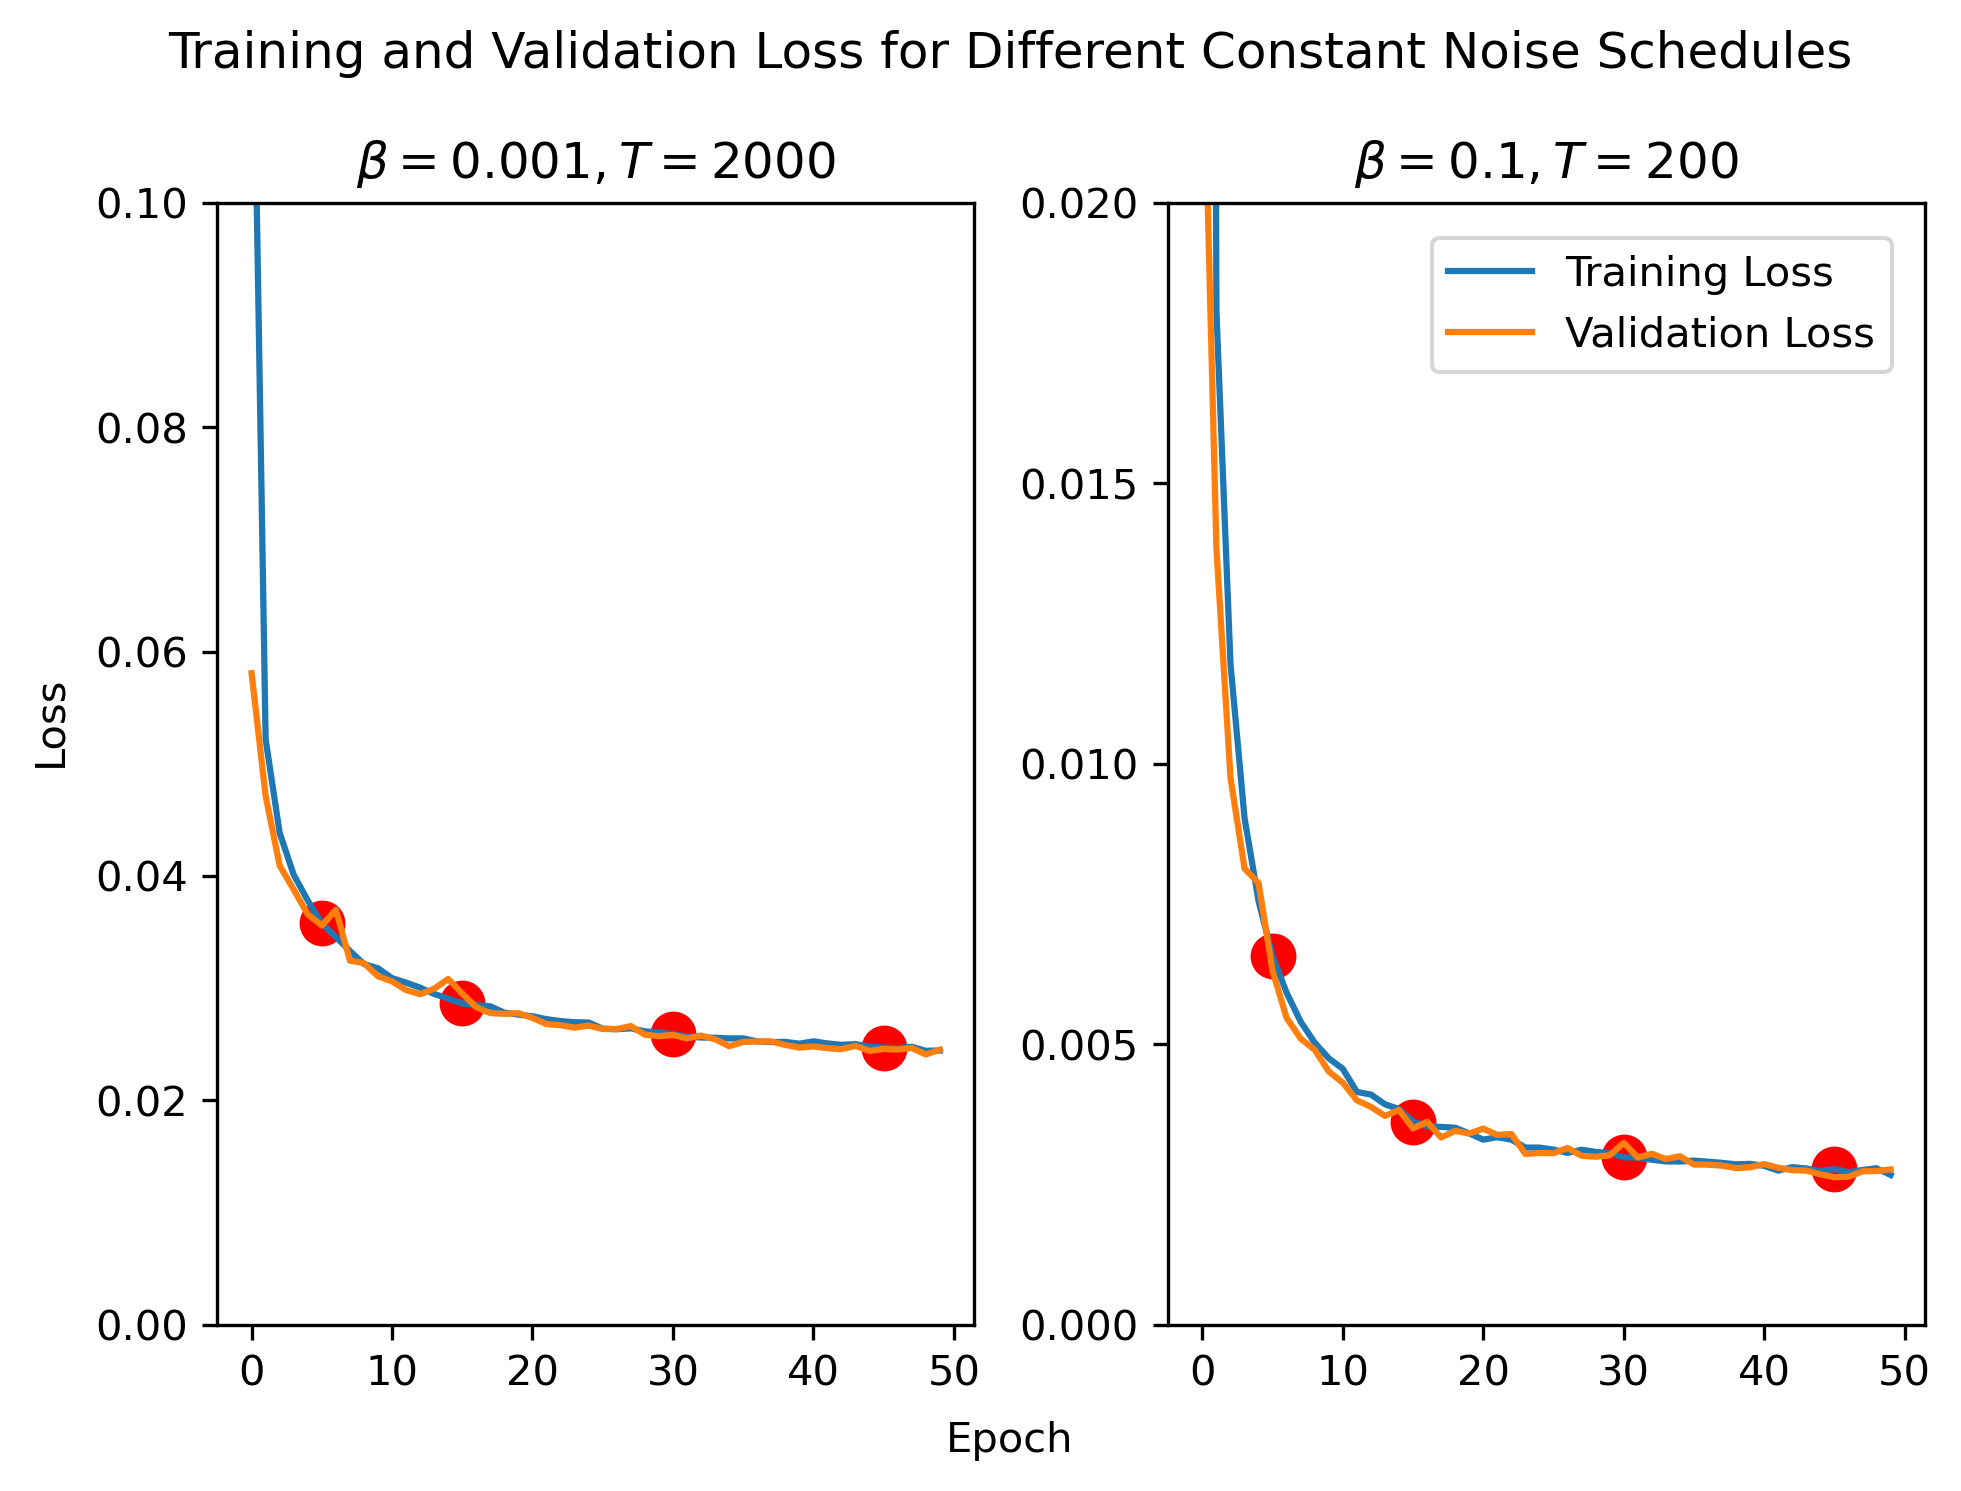
\includegraphics[width=0.8\textwidth]{figs/q1b_loss.png}
    \caption{Training and validation loss curves of the two runs. Training loss shown in blue, validation loss in orange. Red dots indicate epochs 5, 15, 30 and 45.}
    \label{fig:q1b_loss_curves}
\end{figure}

The validation loss curves follow the training loss curves closely, indicating that the model is not overfitting.
\subsubsection{Quality of samples}
From the loss curves alone it would appear that the larger $\beta$ model is performing better. However, the loss curves do not tell the whole story. Figures \ref{fig:train_conditional_samples} and \ref{fig:train_unconditional_samples} show the samples generated by the model at epochs 5, 15, 30 and 45. The samples generated by the model with the smaller $\beta$ value are of obviously of higher quality. Further, the model with the larger $\beta$ does not seem to be training well, with its conditional and unconditionally generated samples showing little improvement over the epochs. This is likely due to the fact that the reverse distributions $Pr(\mathbf{z_{t-1}}|\mathbf{z_{t}})$ are not well approximated by a normal distribution for large $\beta_t$ values as the noise added at each step is too large.

\begin{figure}[H]
    \centering
    \begin{minipage}{0.48\textwidth}
        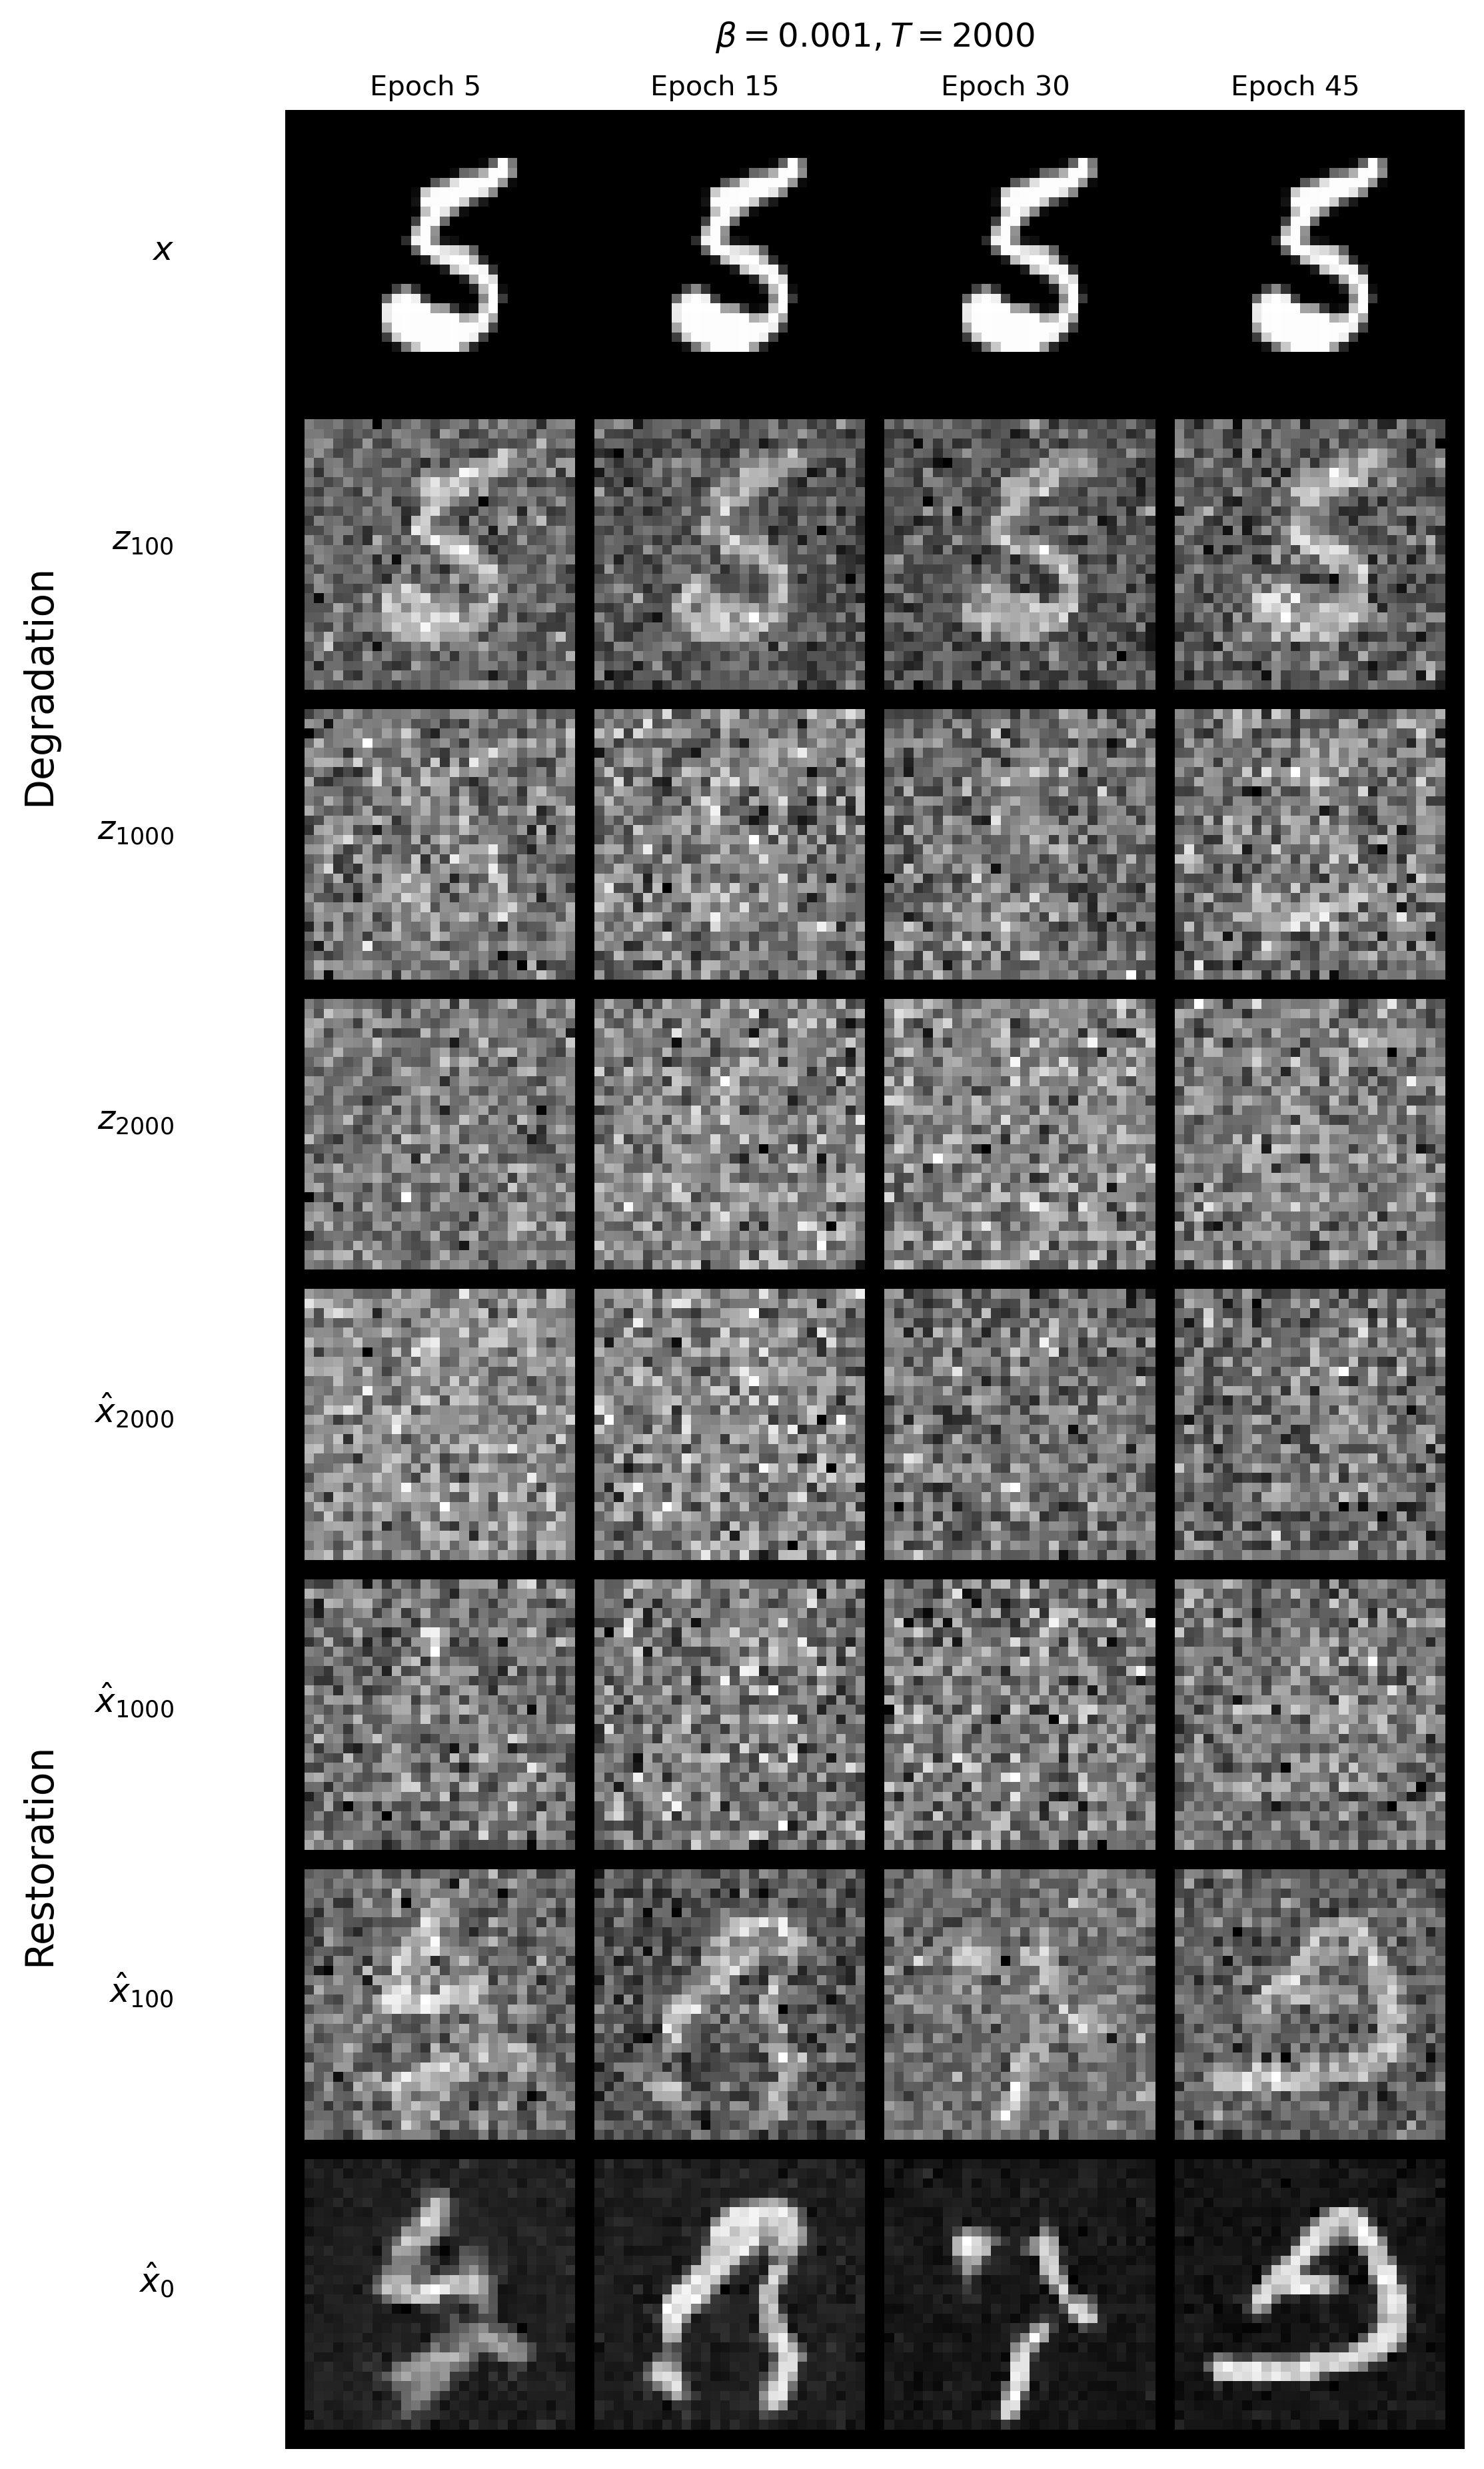
\includegraphics[width=\linewidth]{figs/q1b_good_cond_samples.png}
        \label{fig:train_cond_left_img}
    \end{minipage}\hfill
    \begin{minipage}{0.48\textwidth}
        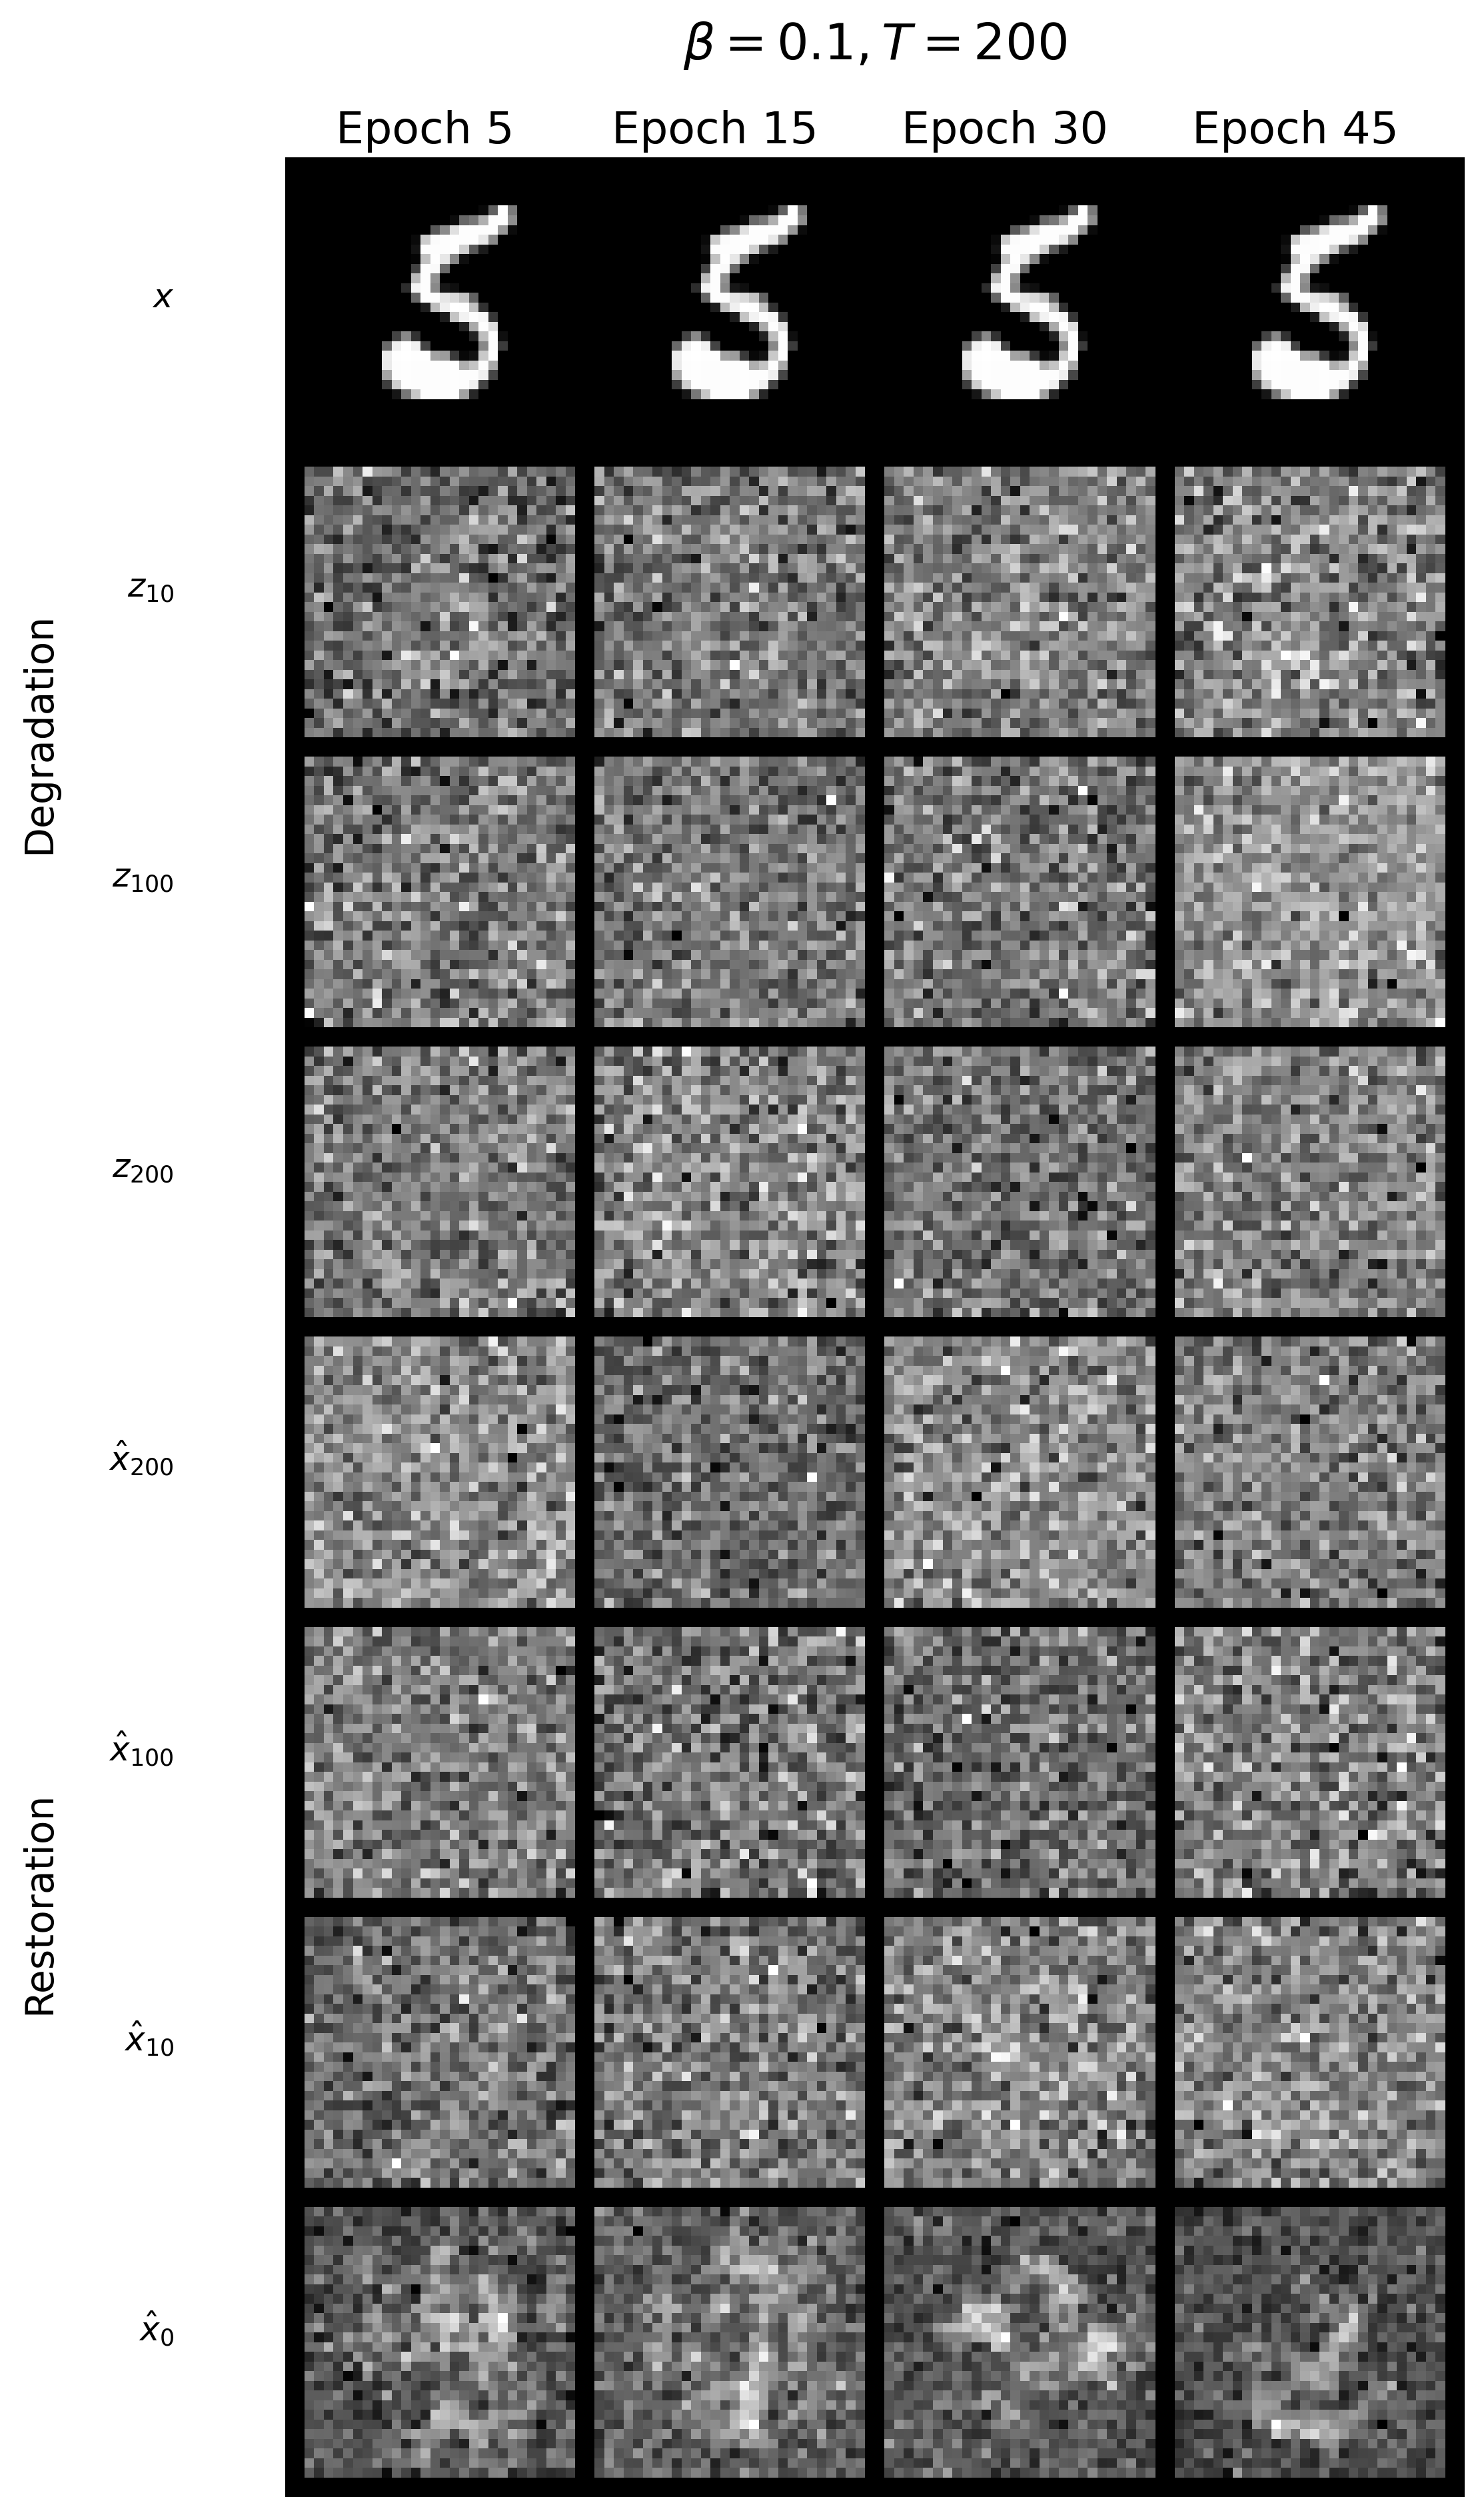
\includegraphics[width=\linewidth]{figs/q1b_bad_cond_samples.png}
        \label{fig:train_cond_right_img}
    \end{minipage}
    \caption{Conditionally generated samples as a function of epoch. $\beta=0.001, T=2000$ model shown on the left and $\beta=0.1, T=200$ shown on the right. The y axis shows the degraded latent variable $z_t$ at 3 times and the reconstructions denoted by $x_t$ at the same times along with the initial image $x$ (first row) and the final reconstructions $\hat{x}$ (last row).}
    \label{fig:train_conditional_samples}
\end{figure}

\begin{figure}[H]
    \centering
    \begin{minipage}{0.48\textwidth}
        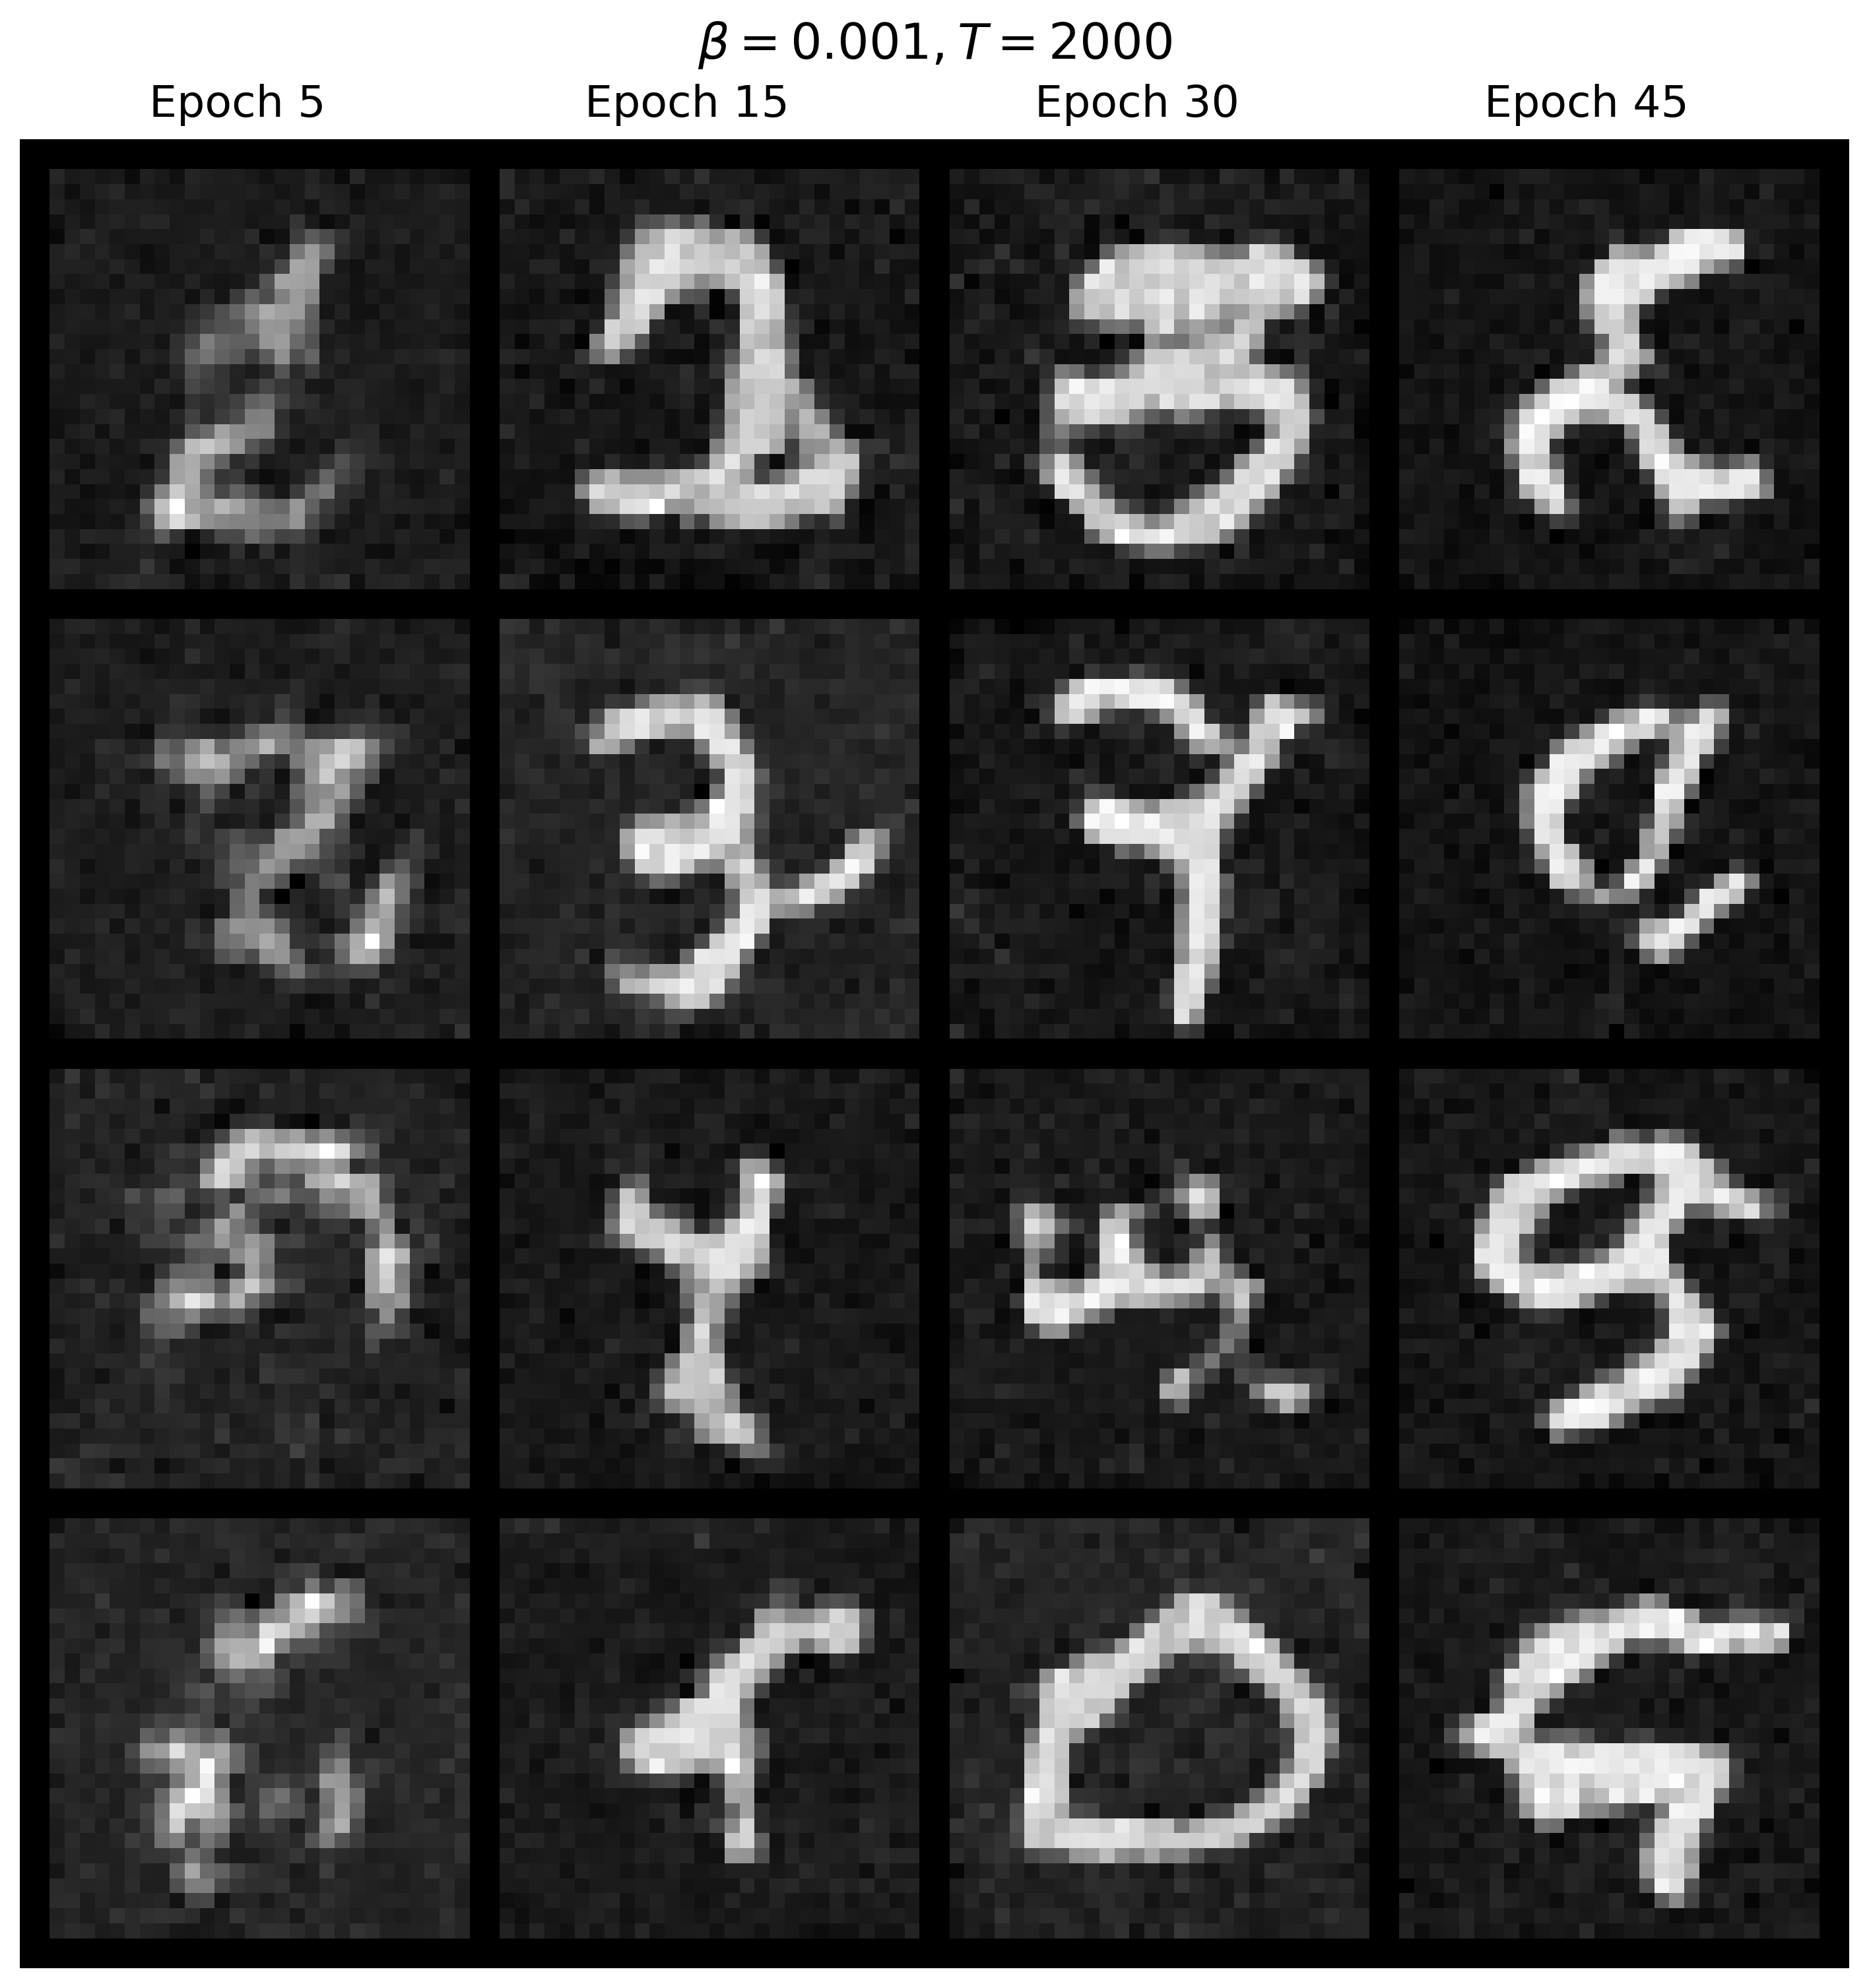
\includegraphics[width=\linewidth]{figs/q1b_good_uncond_samples.png}
        \label{fig:train_uncond_left_img}
    \end{minipage}\hfill
    \begin{minipage}{0.48\textwidth}
        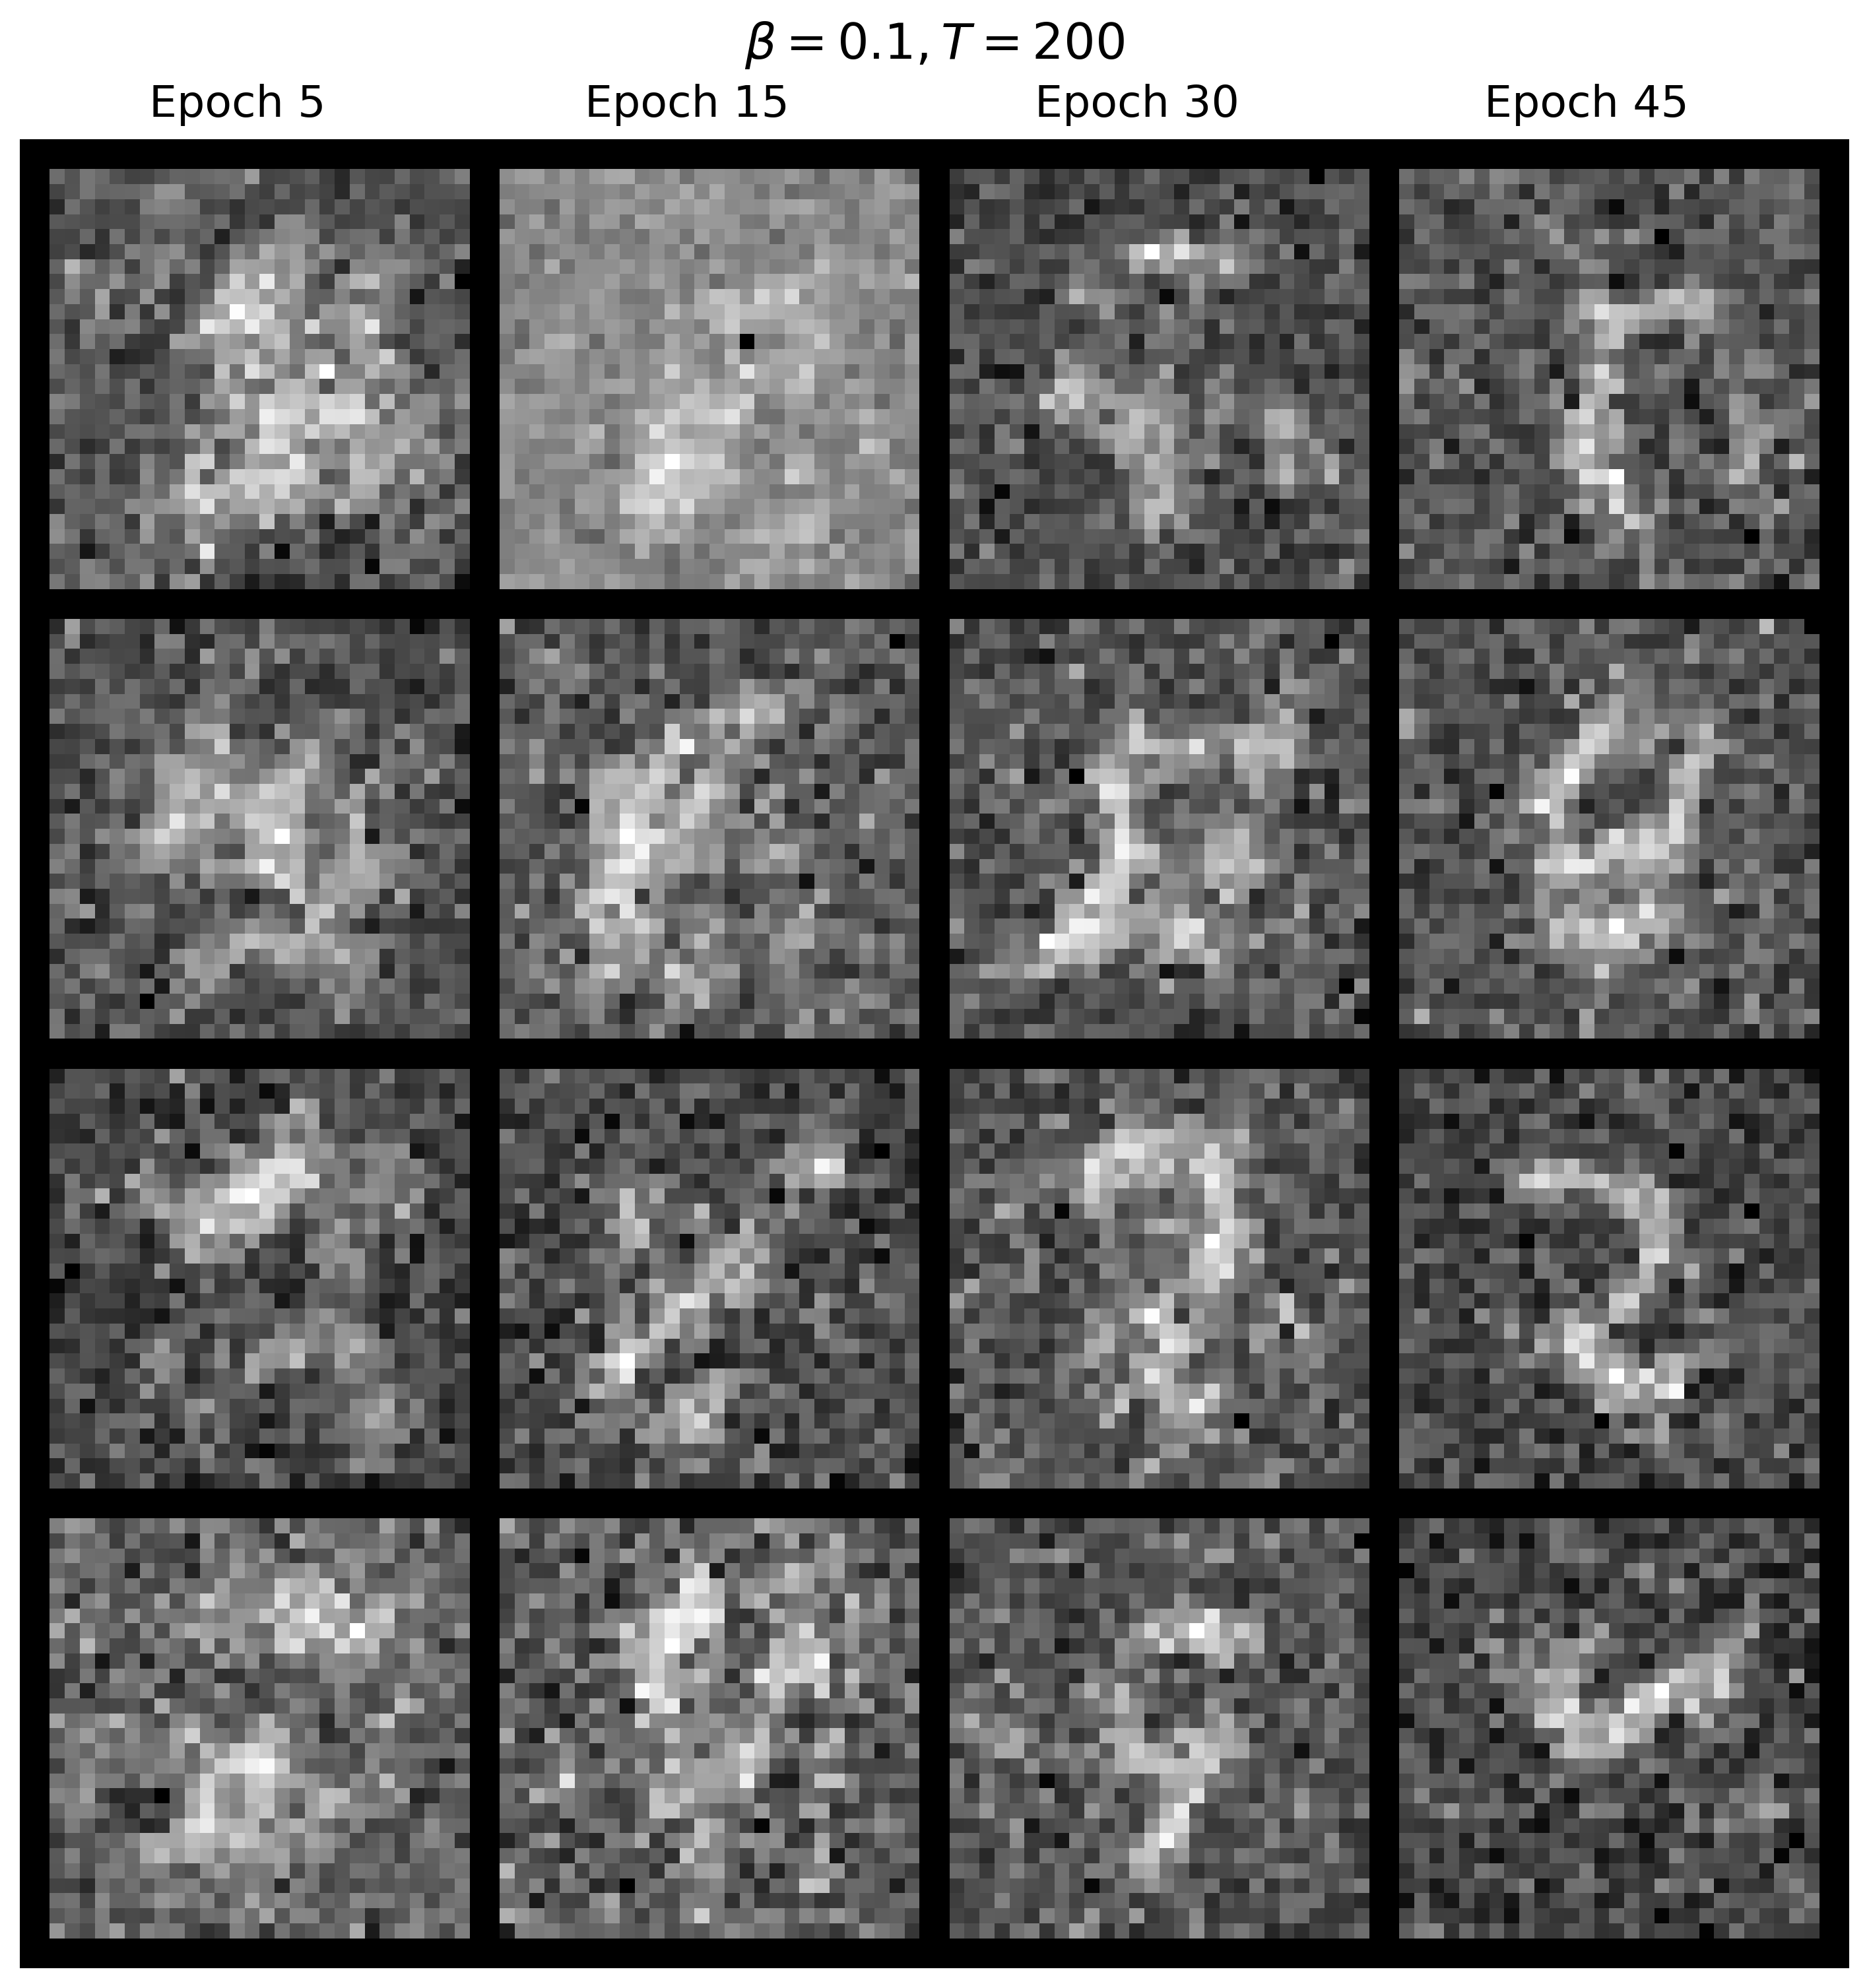
\includegraphics[width=\linewidth]{figs/q1b_bad_uncond_samples.png}
        \label{fig:train_uncond_right_img}
    \end{minipage}
    \caption{Unconditionally generated samples with the good $\beta=0.001$ value (left) and the bad $\beta=0.1$ value (right), shown as a function of the number of epochs.}
    \label{fig:train_unconditional_samples}
\end{figure}
\subsection{Evaluation}
The best model for each noise schedule was selected based on the validation loss and is compared for a final evaluation using the FID score \cite{Fid}, average test loss, average RMSE, average SSIM \cite{ssim}, and average PSNR. The results are summarised in the table \ref{tab:q1b_model_comparison} below. It is worth noting the FID score is calculated using unconditionally generated samples whereas the other metrics are evaluating using conditionally generated samples. Further, while the test loss shows the MSE between the estimated noise and the true noise, the other metrics compare the generated images directly with the images from the MNIST dataset. The FID scores are computationally expensive to calculate and so were calculated over a batch of 1000 samples. The other metrics were calculated over the entire test set of 10000 samples. For this reason the FID score is more noisy than the other metrics.
\begin{table}[H]
    \centering
    \caption{Comparison of Model Performances}
    \begin{tabular}{l|lllll}
    \hline
    Model          & FID Score           & Avg Test Loss        & Avg RMSE           & Avg SSIM         & Avg PSNR           \\ \hline
    Low $\beta$, High $T$ & \textbf{233}    & 0.0245              & \textbf{0.306}            & \textbf{0.164} & \textbf{10.5}    \\
    High $\beta$, Low $T$  & 432             & \textbf{0.00275}     & 0.402  & 0.0336          & 7.94              \\ \hline
    \label{tab:q1b_model_comparison}
    \end{tabular}
    \end{table}

    \begin{figure}[H]
        \centering
        \begin{minipage}{0.48\textwidth}
            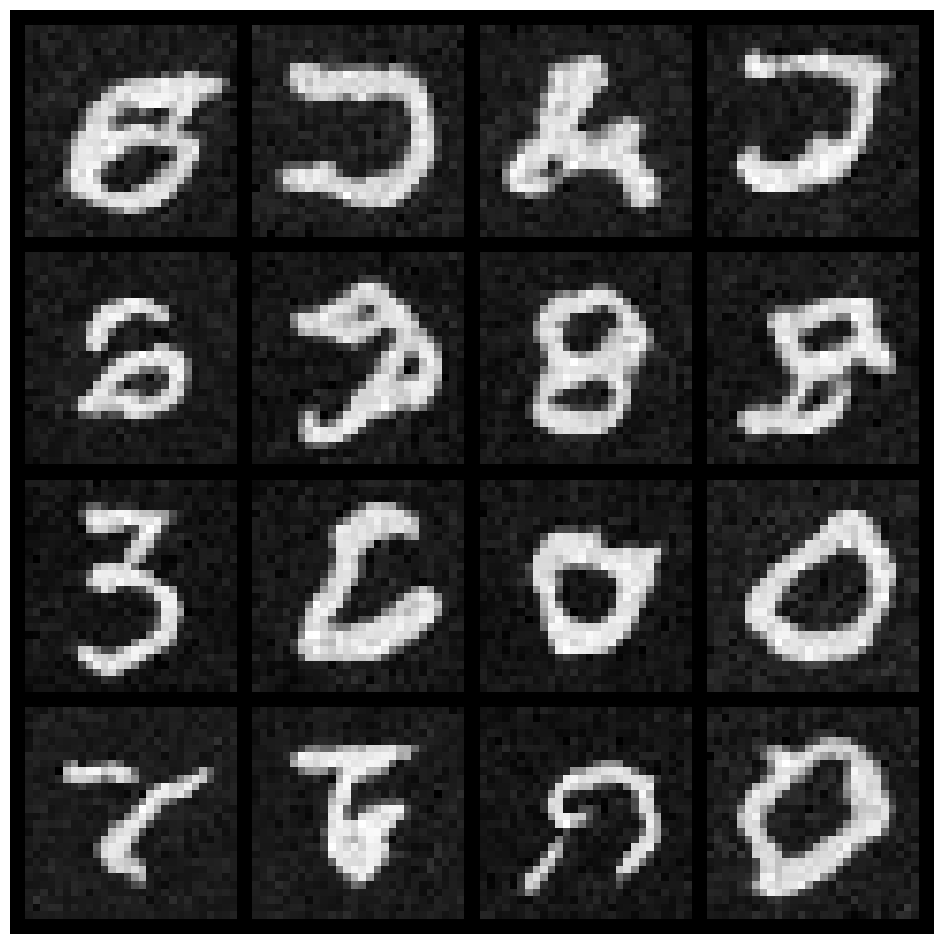
\includegraphics[width=\linewidth]{figs/q1c_good_uncond_samples.png}
            \label{fig:left_img_2}
        \end{minipage}\hfill
        \begin{minipage}{0.48\textwidth}
            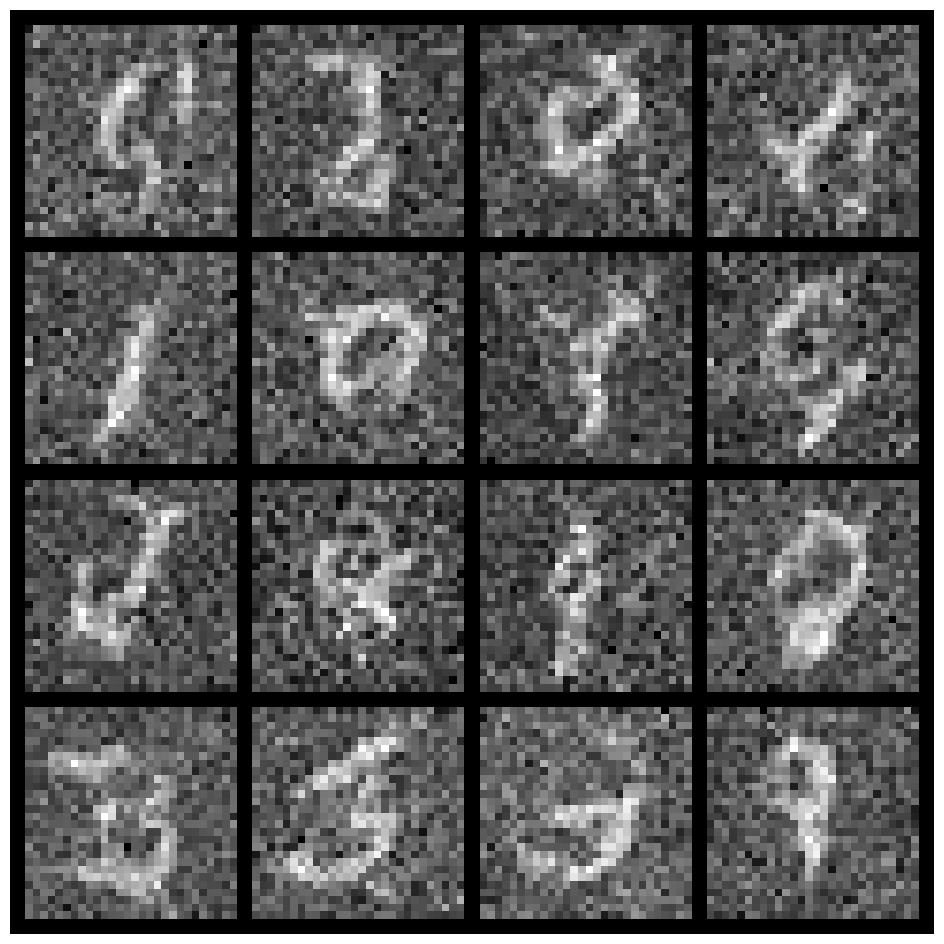
\includegraphics[width=\linewidth]{figs/q1c_bad_uncond_samples.png}
            \label{fig:right_img_2}
        \end{minipage}
        \caption{64 Unconditionally generated samples for the model $\beta = 0.001, T=2000$ (left) and the bad model  $\beta = 0.1, T=200$ (right).}
        \label{fig:q1c_unconditional_samples}
    \end{figure}

The model with the smaller $\beta$ value performs better across all metrics, with the exception of the average test loss. The FID score is significantly lower for the model with the smaller $\beta$ value, indicating that the generated samples are more similar to the reference dataset.  To further illustrate the differences between the two models, 64 samples are unconditionally generated and are shown in figure \ref{fig:q1c_unconditional_samples}. The samples generated by the model with the smaller $\beta$ value are of higher quality. Interestingly, the model with a higher $\beta$ value records a lower average test loss, a phenomenon that becomes clear when examining the noise schedules depicted in Figure \ref{fig:q1c_noise_schedules}.
\begin{figure}[H]
    \centering
    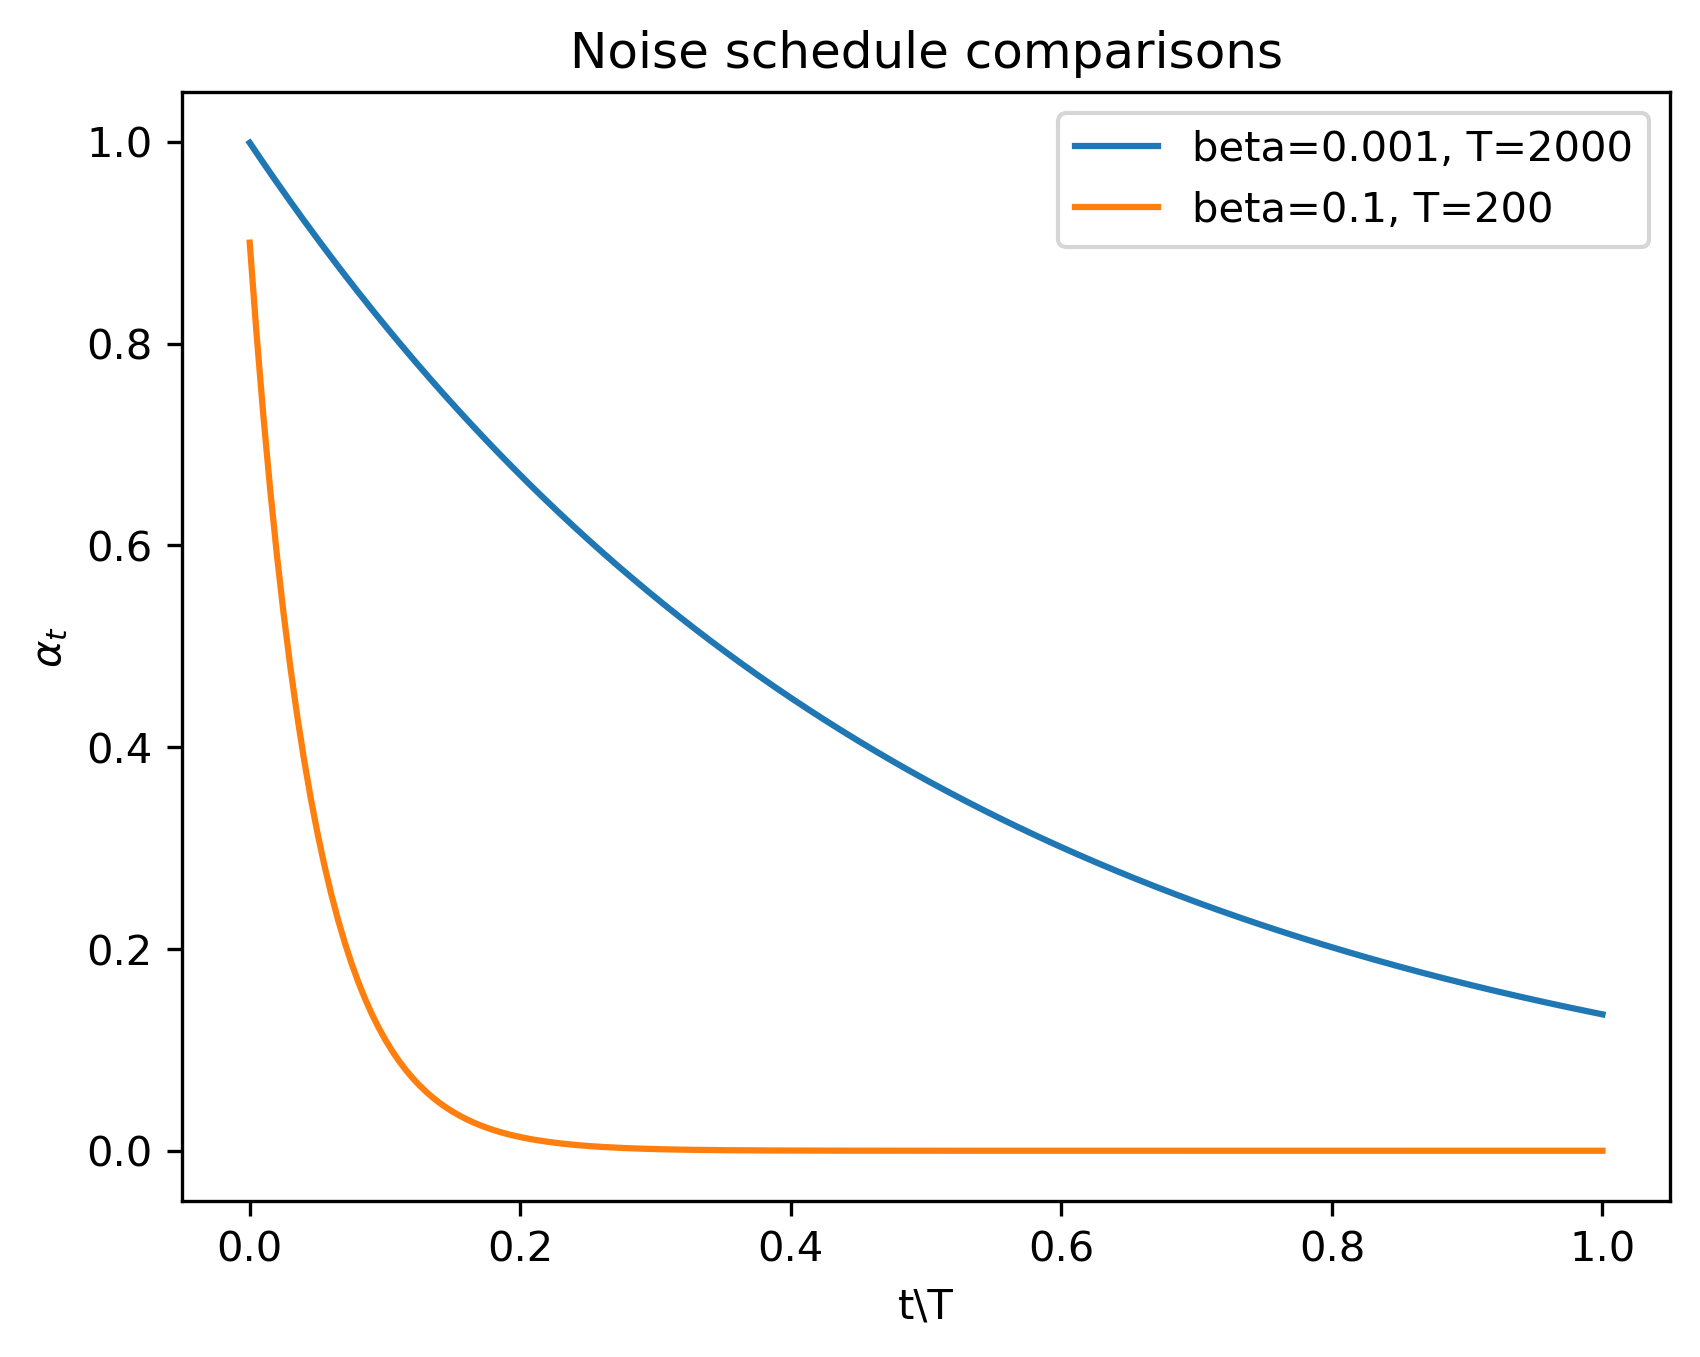
\includegraphics[width=0.5\textwidth]{figs/q1c_noise_schedule_comparison.png}
    \caption{Comparison of the noise schedules for the two models.}
    \label{fig:q1c_noise_schedules}
\end{figure}
The rapid decay of $\alpha_t$ for the larger $\beta$ value means that most of the latent variables $\mathbf{z_t}$ are almost entirely defined by the noise $\boldsymbol{\epsilon_t}$. This leads the model to effectively disregard the input image $\mathbf{x}$, opting instead to mimic the identity function to minimise the Mean Squared Error (MSE). Which means it fails to learn the data's underlying distribution. This scenario underscores that a lower test loss is not always indicative of meaningful learning or enhanced model performance. Figure \ref{fig:q1c_noise_schedules} also reveals another interesting result. Even though the model with the smaller $\beta$ does not achieve an $\alpha_T$ value of zero (approximately 0.13), it still successfully generates high-quality samples with $\mathbf{z_T}$ sampled from a standard normal distribution. This indicates that one does not need to approximate the latent distribution $Pr(\mathbf{z_T})$ perfectly to generate high-quality samples. This will be further explored in the next section.
\section{Part 2 - Custom Degradations}
\subsection{Prelude - the UNet Decoder}
% Briefly introduce unet as a more powerful decoder. Introduce why its more powerful, the architecture, the time encoding modification.
The diffusion models outlined below transition the decoder's structure from a basic CNN architecture to a more powerful UNet architecture. Further, the time embedding mechanism is also changed. Now they are generated via the sinusoidal positional embedding method introduced by Vaswani et al in their original paper on the Transformer \cite{vaswani2023attention}. The time embeddings are also added to the feature maps at each layer, rather than just the first as was the case previously.
The UNet architecture used is adopted from the original implementation by Bansal et al. in their presentation of cold diffusion models \cite{bansal2022cold}. Here, the UNet is implemented using \texttt{torch.nn.Functional.layer\_norm} instead of the custom \texttt{LayerNorm} class in the original. It is also applied after the main convolutional layers of the ConvNext block \cite{liu2022convnet}, before the residual connection is added. This was found to give better performance.
% Describe the modified decoder net
\subsection{The Role of Gaussian Noise}
% Explain the role of noise and what happens when eps is not Gaussian or even random var.
Before discussing diffusion models with custom degradations, understanding the role of Gaussian noise in the foundational theory of diffusion probabilistic models (DDPMs) is crucial. In the original framework, noise $\boldsymbol{\epsilon}$ is drawn from a standard normal distribution which means the latent variable $\mathbf{z_t}$ is also a random variable that follows a normal distribution. Specifically, the distributions of the random variables are defined as:
$$
q(\mathbf{z_t}|\mathbf{z_{t-1}}) = \mathcal{N}(\sqrt{1-\beta_t}\mathbf{z_{t-1}}, \beta_t \mathbf{I}).
$$
Or using the direct update rule in \ref{eq:z_t_alpha_gauss_noise}:
$$
q(\mathbf{z_t}|\mathbf{x}) = \mathcal{N}(\sqrt{\alpha_t}\mathbf{x}, \alpha_t\mathbf{I}).
$$
Because these distributions have the form of a normal distribution, it can be shown that the conditional distribution $q(\mathbf{z_{t-1}}|\mathbf{z_t}, \mathbf{x})$ is also normal and the reverse distributions $Pr(\mathbf{z_{t-1}}|\mathbf{z_t})$ can be well approximated by normal distributions in the limit of a small $\beta_t$ and large $T$. This is a key assumption in the derivation of the loss function in \ref{eq:loss_function}. For the full derivation see chapter 18 of Prince \cite{prince}. If the noise $\boldsymbol{\epsilon}$ is not sampled from a normal distribution, the reverse distributions $Pr(\mathbf{z_{t-1}}|\mathbf{z_t})$ will not be normal or even a distribution at all in the case of deterministic degradations. This means the loss function will no longer have any probabilistic grounding to be linked with maximising the likelihood of the data, therefore it is not obvious that such a model would be trainable, let alone generate high quality samples. This is the context behind the following experiment.

\subsection{Gaussian Blur Custom Degradation}
To explore a degradation which contrasts with the Gaussian noise used in the original DDPM, a Gaussian blur degradation is introduced. This is a deterministic
degradation where the degradation operator is defined as:
\begin{equation}
    \mathbf{z_t} = G_t * \mathbf{z_{t-1}} = G_t * \dots * G_1 * \mathbf{x} = \tilde{G}_t * \mathbf{x}
\end{equation}
where $G_t$ is a Gaussian blur kernel of variance $\sigma_t^2 = \beta_t$ and $\tilde{G}_t$ is the convolution of all the kernels up to time $t$. The sampling algorithm defined in algorithm \ref{alg:sampling} is replaced with the one introduced by Bansal et al in cold diffusion \cite{bansal2022cold}.

In general, there are only 3 known conditions a custom degradation must satisfy to be used to train a diffusion model.
First, the degradation must be a smooth function of $t$. Second, the degradation must return the original image when $t=0$. Lastly, the latent $\mathbf{z_T}$ must be unique for each input. Gaussian blurs clearly satisfy the first 2 conditions. The 3rd condition translates to the statement that the mean of the input image is a unique identifier of that image, which is not necessarily true as two images can share the same mean, however in practice, given enough precision in the mean calculation and a large enough dimensionality of $\mathbf{x}$, this is a reasonable assumption.

% D for Gaussian blur. Details of the degradation, how it is implemented
\subsection{Training details}
The model was trained on the MNIST dataset for 50 epochs with a batch size of 128. The training and validation datasets were obtained by using an 80:20 split. The model was optimised using ADAM with a learning rate of $2 \times 10^{-4}$. The model was trained with a constant noise schedule of $\beta = 1$ and $T=100$. A kernel of size 11x11 was used for the Gaussian blur degradation. The loss used was the MSE between the output of the decoder and the original image $x$. The decoder model used was the UNet. The UNet was initialised with 32 channels in the first layer with 2 downsampling layers which each double the number of channels of the previous layer.

To generate samples unconditionally, $\mathbf{z_T}$ is initialised as a uniform image, with intensity values sampled from a normal distribution that was fit to the mean intensities of the MNIST training set after 100 blurs. It was found that to obtain a diverse set of samples, a small amount of noise was required to be added to the latent variable $\mathbf{z_T}$. The motivation for this is discussed by Bansal et Al in their cold diffusion paper \cite{bansal2022cold}.
\subsection{Training Analysis}
As before, the training and validation loss curves as presented along with conditional and unconditionally generated samples at epochs 3, 5, 15 and 45. The conditional samples are shown in figure \ref{fig:q2b_conditional_samples} and the unconditional in figure
\ref{fig:q2b_unconditional_samples}.

% figure showing train and val loss curve
\begin{figure}[H]
    \centering
    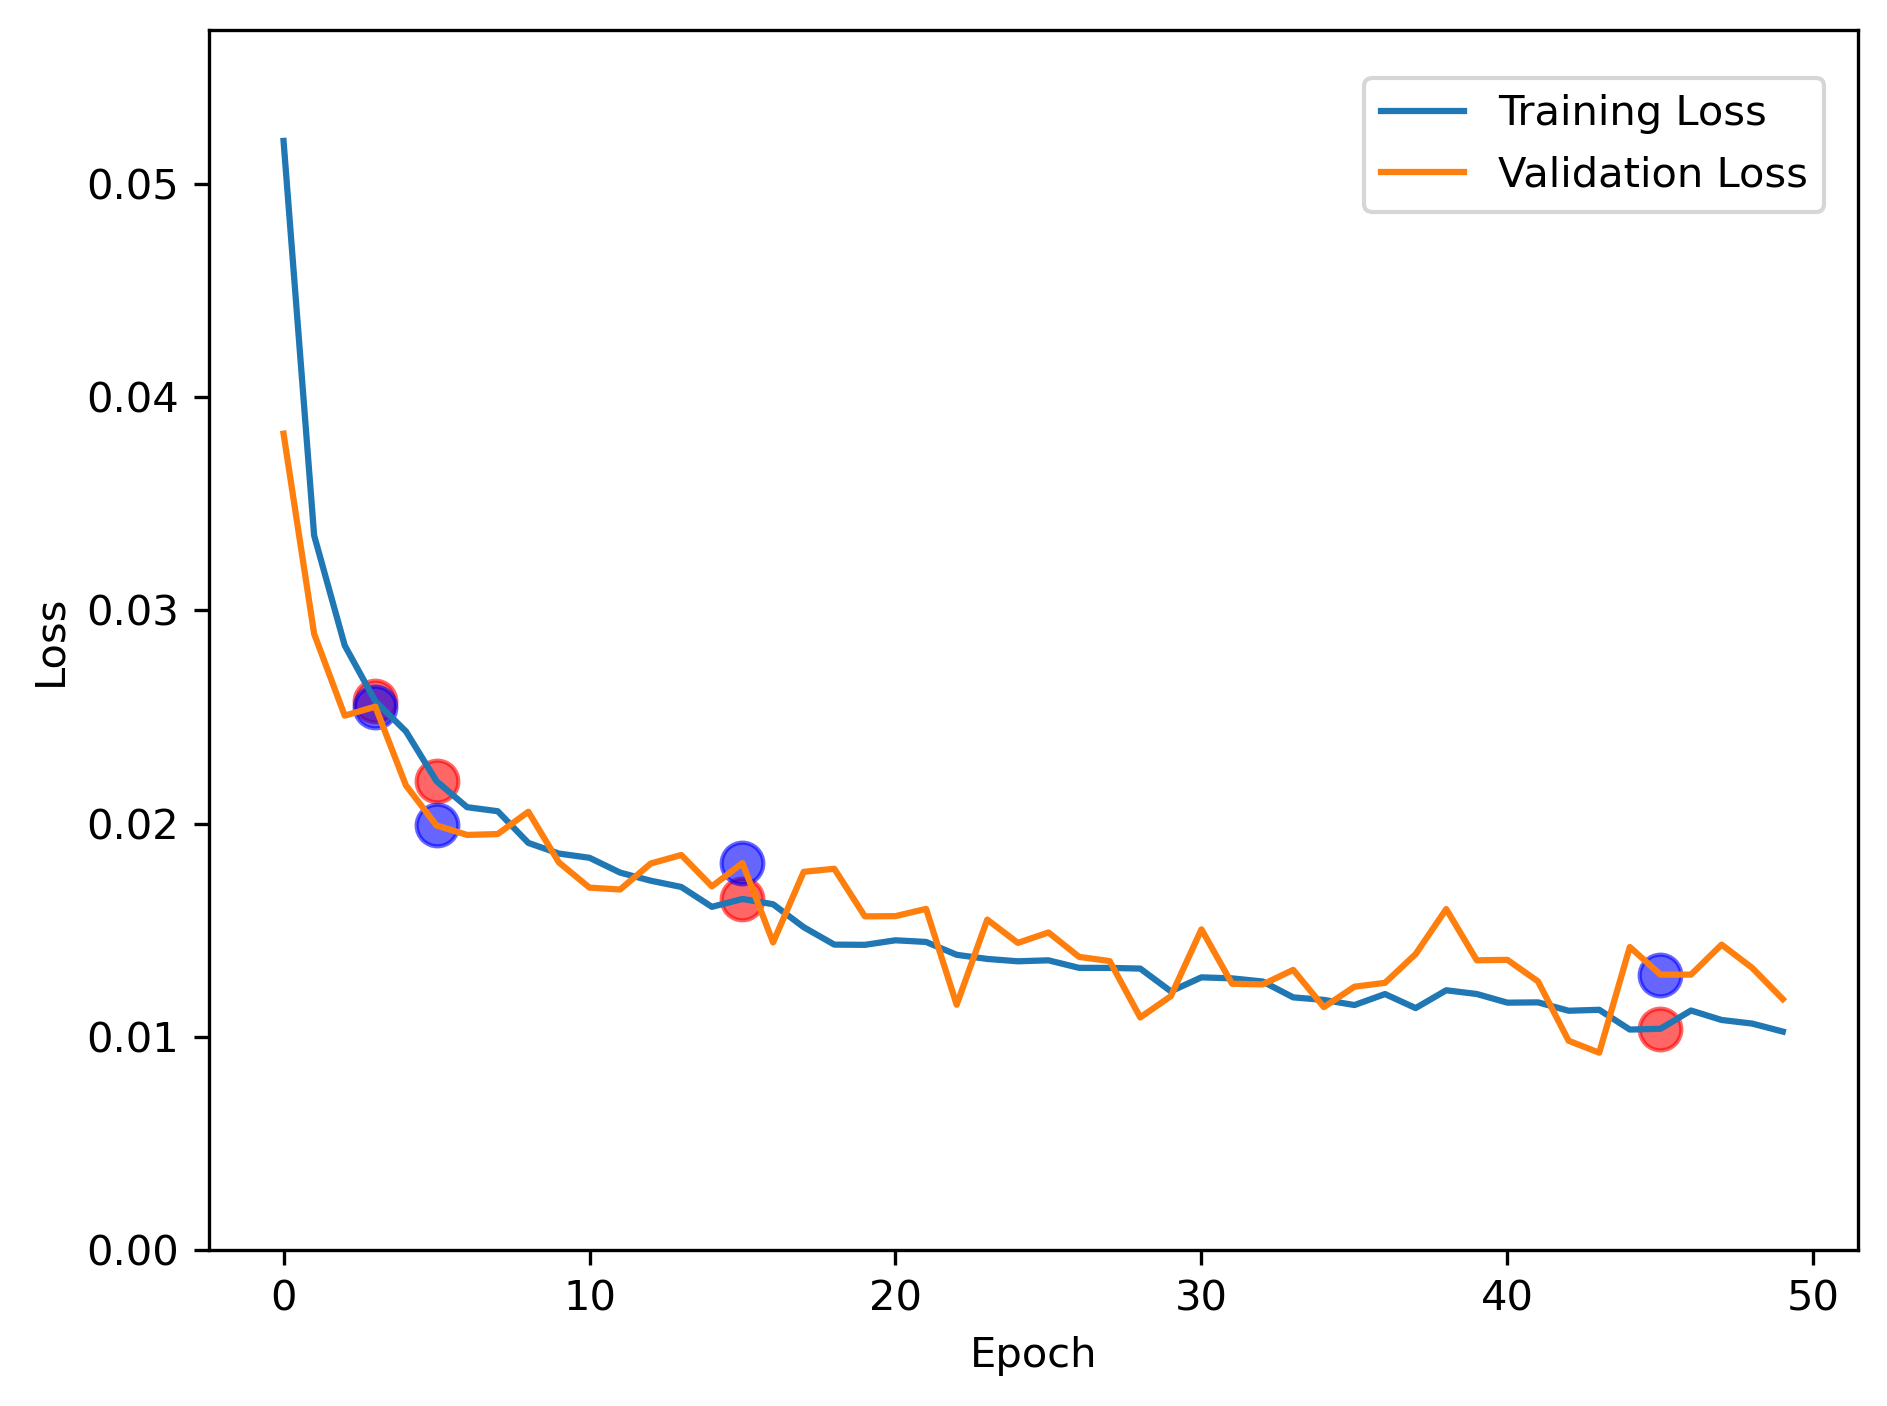
\includegraphics[width=0.8\textwidth]{figs/q2b_blur_loss.png}
    \caption{Training and validation loss curves for the model with Gaussian blur degradation. Blue circles show the training loss and orange circles show the validation loss values for epochs 3, 5, 15, 45 at which samples are generated.}
    \label{fig:q2b_loss}
\end{figure}


From figure \ref{fig:q2b_loss} it is clear that the model is training well. The training and validation loss curves are close together and indicate the model is not overfitting. The conditional samples in figure \ref{fig:q2b_conditional_samples} show that the model is able to generate high quality samples. Both forms of sampling show that the fidelity improves over the epochs with the final epochs featuring very little background noise. The unconditionally generated samples however  in figure \ref{fig:q2b_unconditional_samples} show that while model is able to slightly improve the fidelity of the samples, the diversity does not improve nor do they become more number like. This is interesting because the conditional sampling results shows that the model is capable of generating MNIST-esque samples. This shows the issue lies in the way in which the latent space of $\mathbf{z_T}$ is sampled.

\begin{figure}[H]
    \centering
    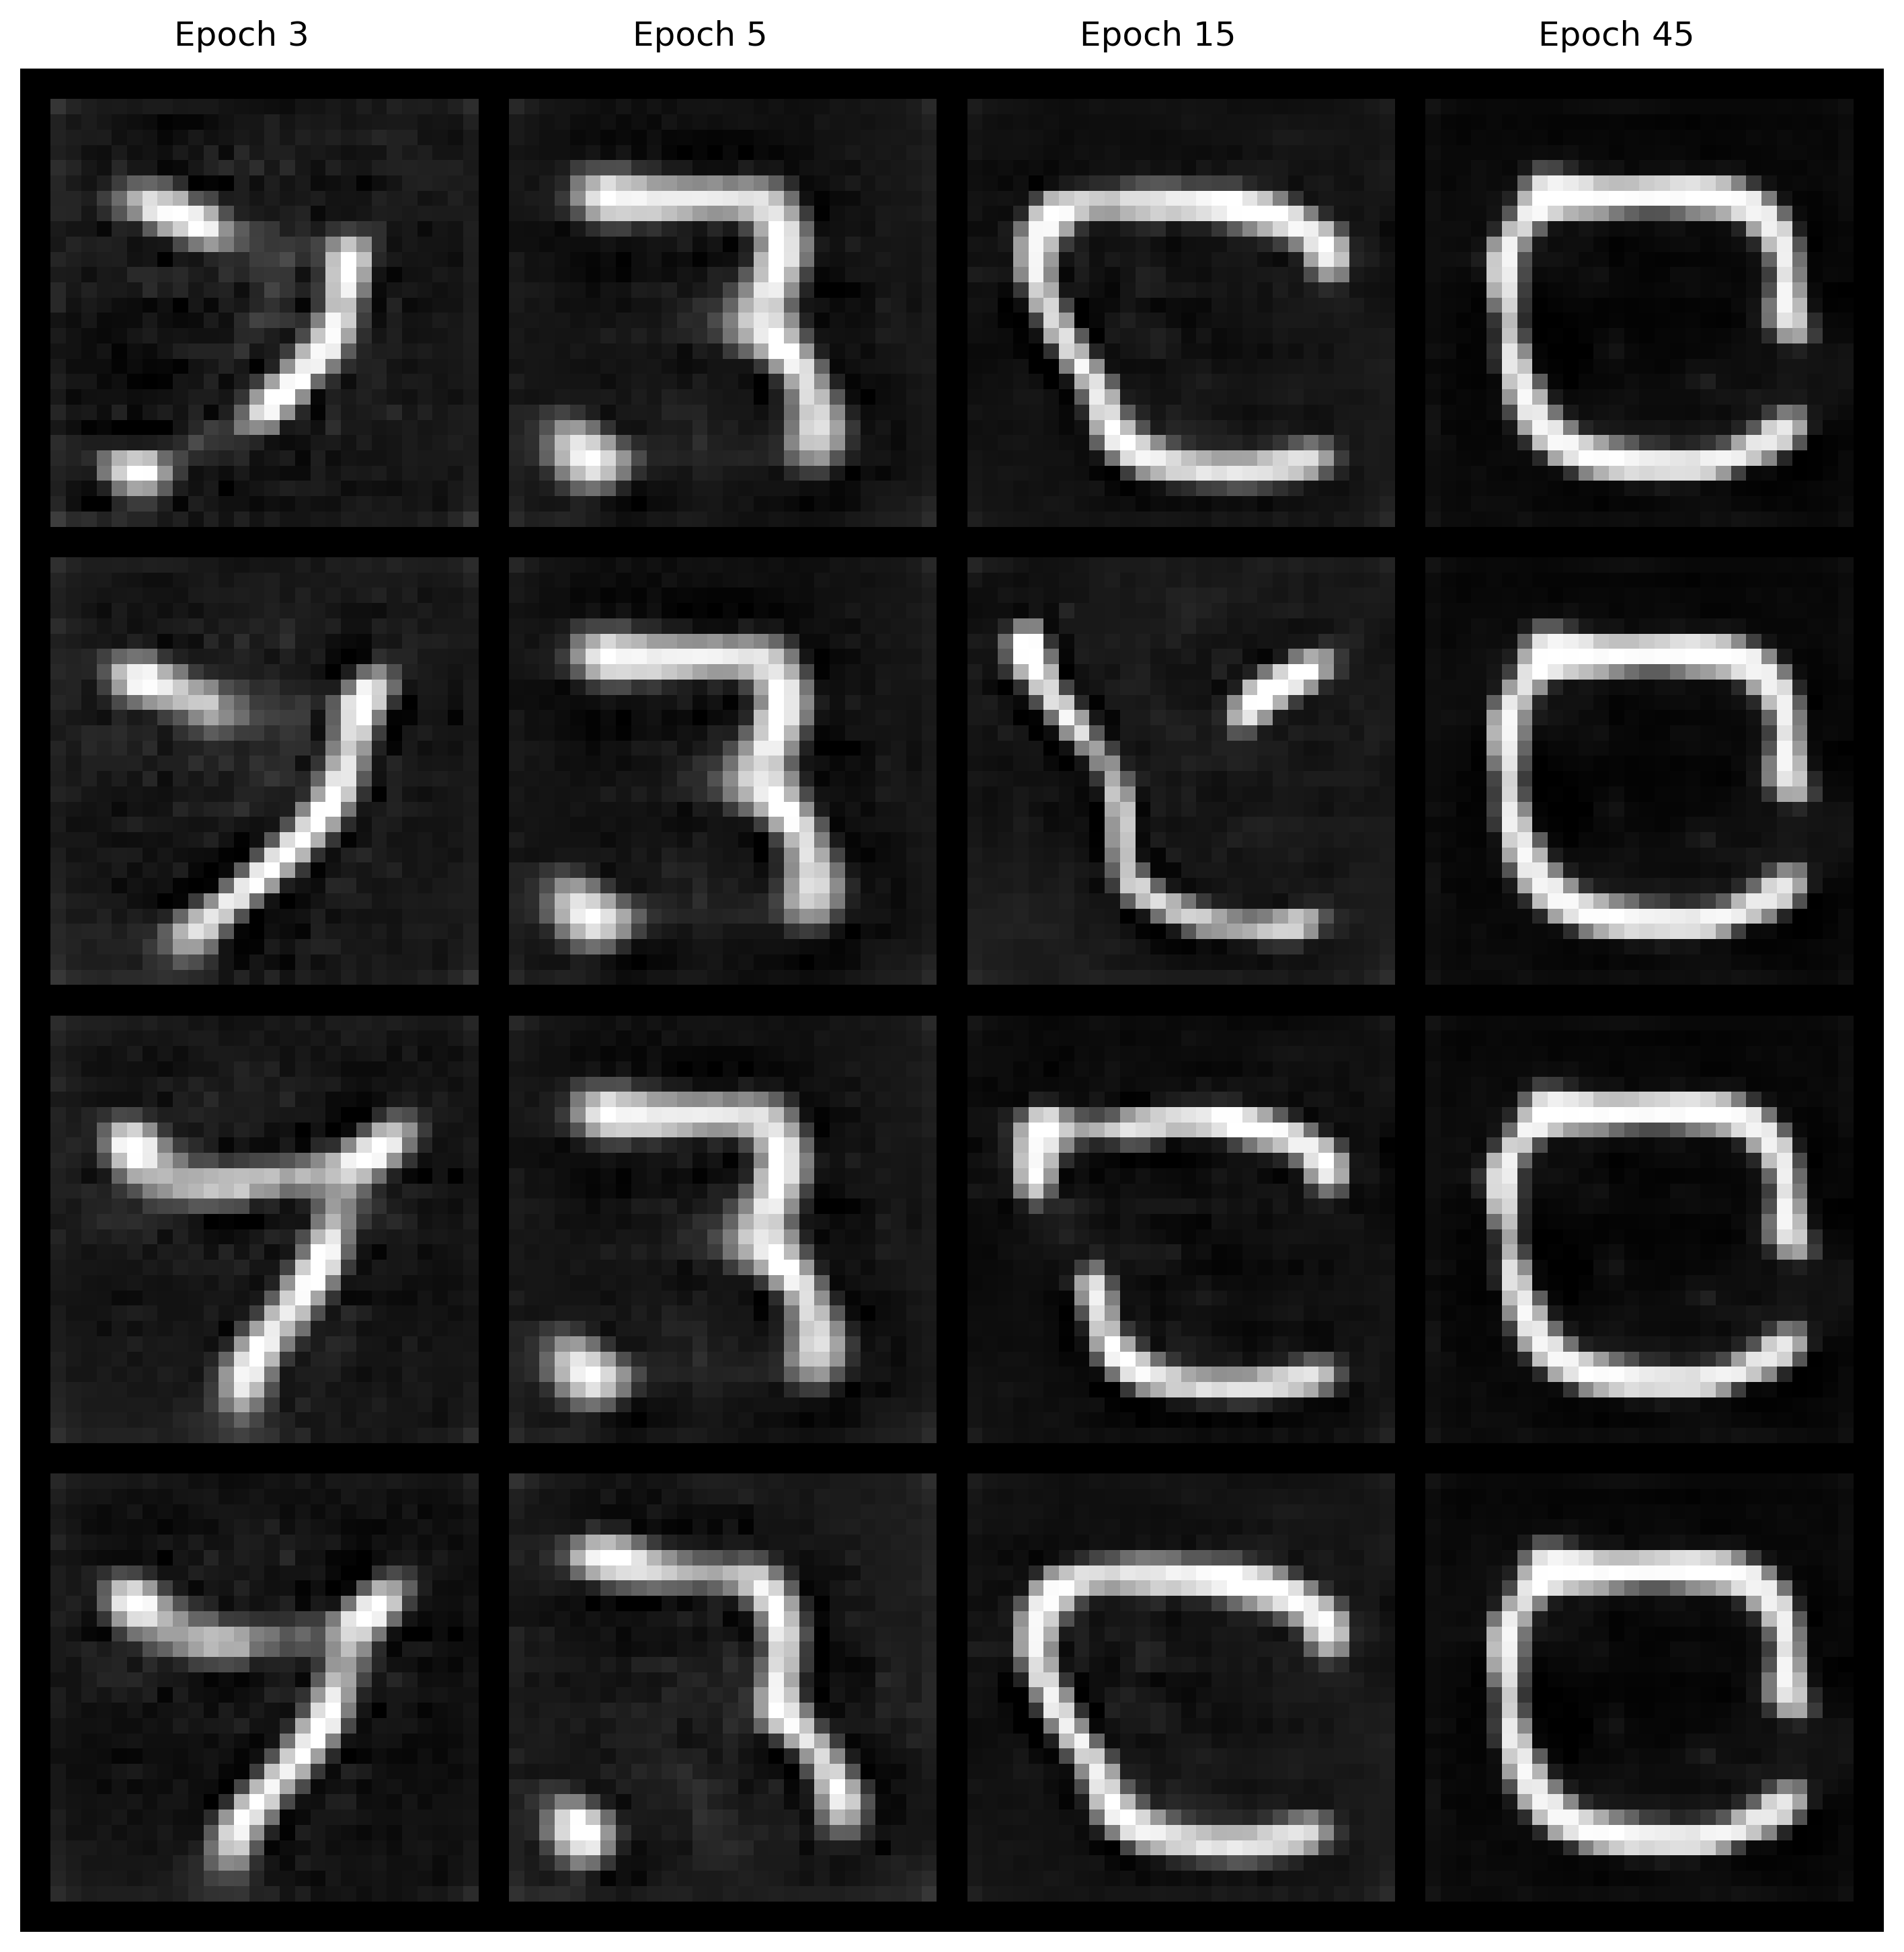
\includegraphics[width=0.8\textwidth]{figs/q2b_blur_uncond_samples.png}
    \caption{Unconditionally generated samples as a function of epoch for the model with Gaussian blur degradation.}
    \label{fig:q2b_unconditional_samples}
\end{figure}

\begin{figure}[H]
    \centering
    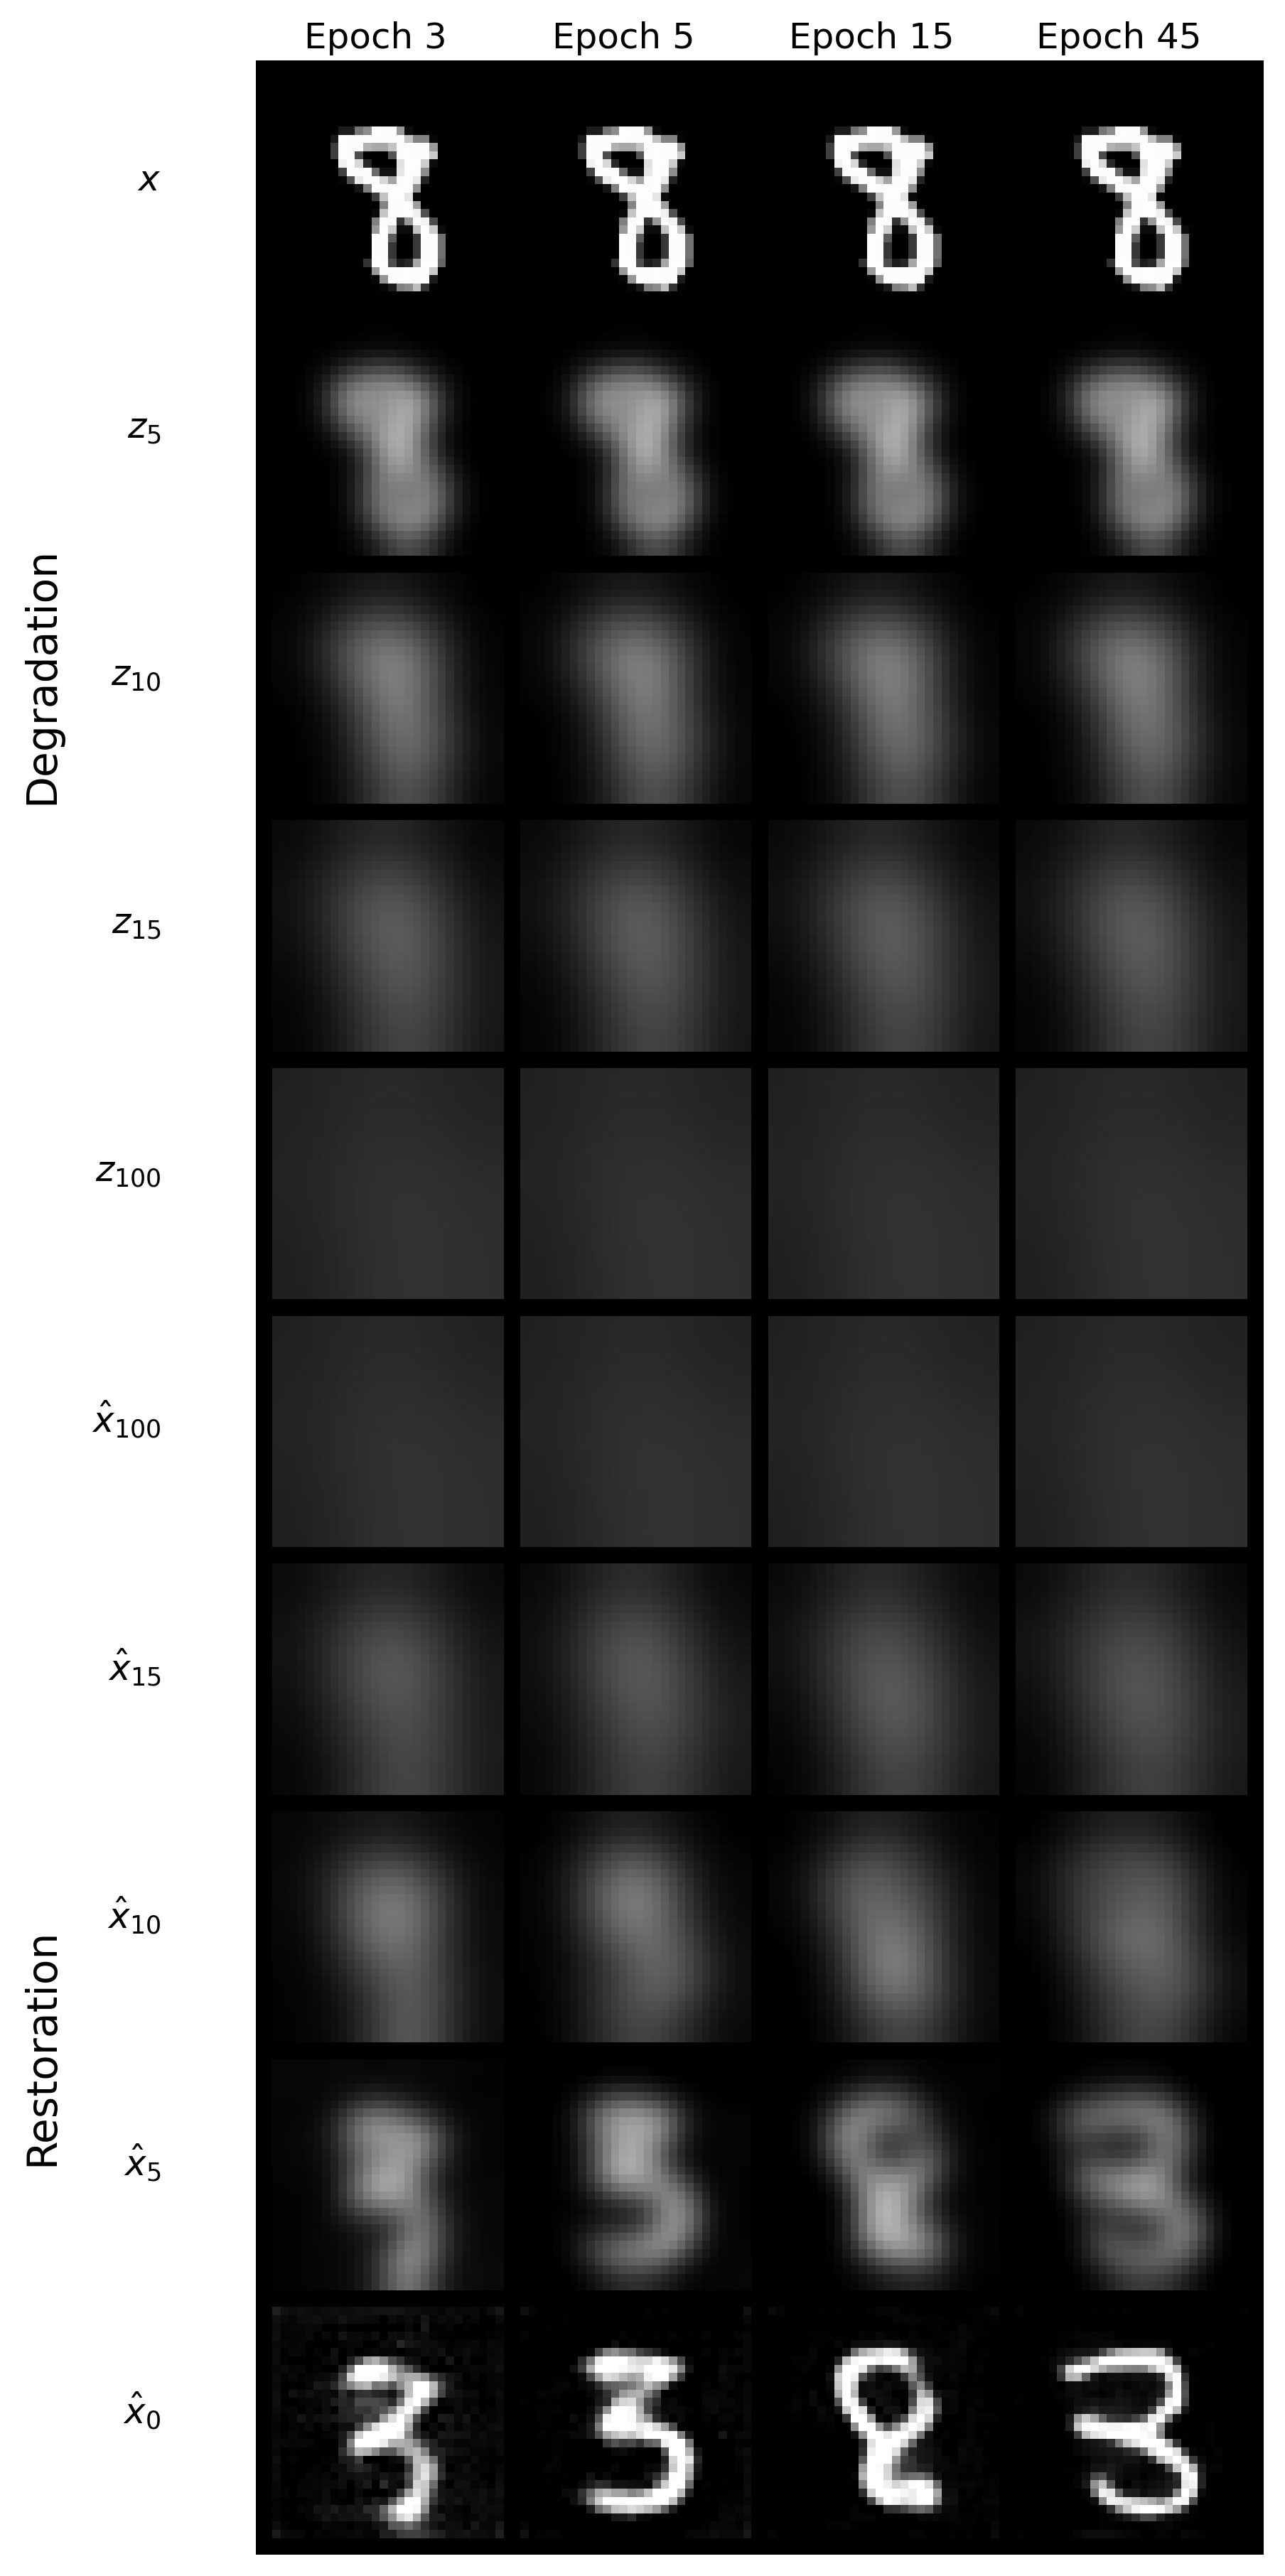
\includegraphics[width=0.6\textwidth]{figs/q2b_blur_cond_samples_norm.png}
    \caption{Conditionally generated samples as a function of epoch for the model with Gaussian blur degradation. The y axis shows the degraded latent variable $z_t$ at 3 times and the reconstructions denoted by $x_t$ at the same times along with the initial image $x$ (first row) and the final reconstructions $\hat{x}$ (last row).}
    \label{fig:q2b_conditional_samples}
\end{figure}


\section{Comparison of Models}
For a fair comparison, the original DDPM model with Gaussian noise degradation is retrained using the same decoder and other hyperparameters with $T=1000$. The model is now trained with a cosine noise schedule as this was found to by Nichol et al to be the best performing noise schedule for this style of model \cite{nichol2021improved}. Conditional and unconditionally generated samples from the two models are compared in figure \ref{fig:q2c_conditional_samples} and \ref{fig:q2c_unconditional_samples} respectively. The model is then evaluated using the previously introduced image quality metrics on 1000 cases from the MNIST test set, the results are summarised in table \ref{tab:q2c_model_comparison}.
\begin{table}[h]
    \centering
    \begin{tabular}{lccccc}
    \hline
    Model & Avg Test Loss & Avg RMSE & Avg SSIM & Avg PSNR & FID Score \\
    \hline
    Gaussian Blur Diffusion & \textbf{0.0113} & \textbf{0.2312} & \textbf{0.3549} & \textbf{13.2237} & 304.0255 \\
    DDPM Gaussian Noise & 0.0271 & 0.3592 & 0.0804 & 9.0724 & \textbf{172.6256} \\
    \hline
    \end{tabular}
    \caption{Performance Comparison of Gaussian Blur Diffusion Model vs DDPM Gaussian Noise Model. Bold indicates the best performing model for each metric.}
    \label{tab:q2c_model_comparison}
\end{table}

All metrics except the FID score show that the Gaussian blur model outperforms the DDPM model. The FID score for the Gaussian blur model is artificially inflated due to the fact they were calculating using samples that were generated unconditionally which are not of high quality. This was done to reduce the computational cost of calculating the score. This discrepancy can clearly be seen in fig \ref{fig:q2c_unconditional_samples}. The Gaussian noise model is able to generate a more diverse set of samples unconditionally compared to the Gaussian blur model.
\begin{figure}[ht]
    \centering
    \begin{subfigure}{.4\textwidth}
        \centering
        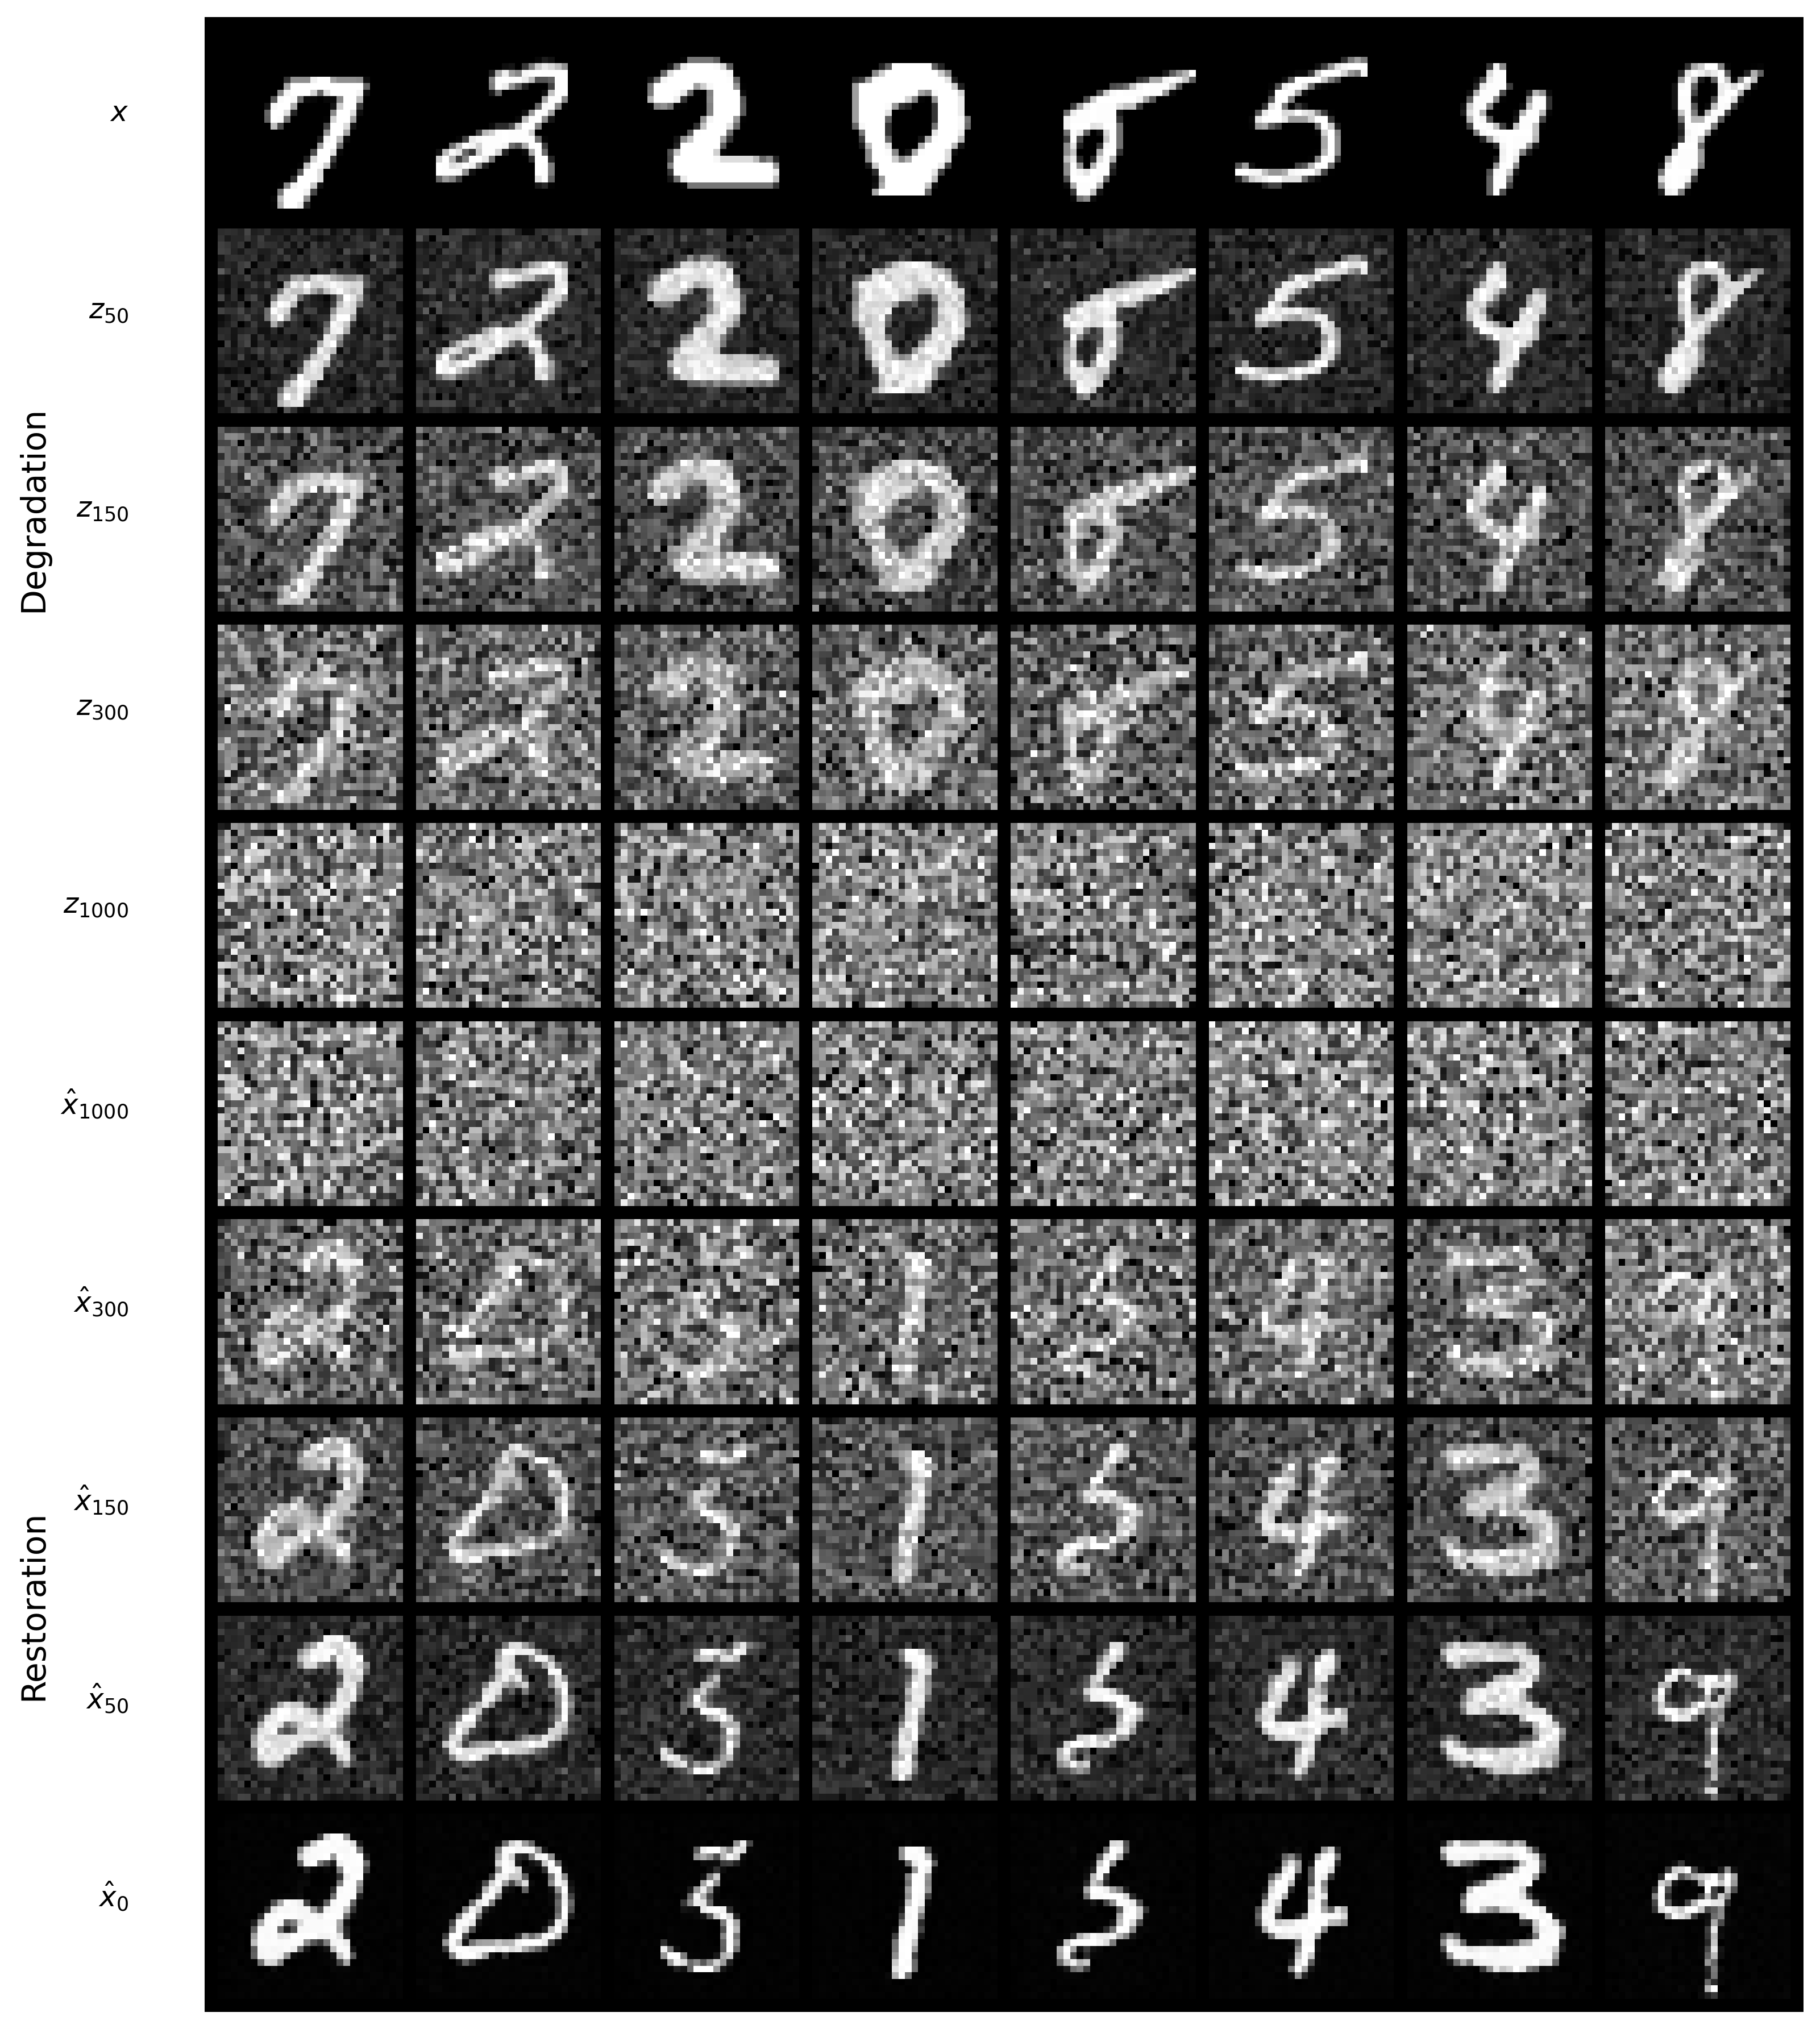
\includegraphics[width=0.9\linewidth]{figs/q2c_ddpm_cond_samples_norm_8.png}
        \caption{Gaussian noise model.}
        \label{fig:cond_ddpm}
    \end{subfigure}%
    \hfill
    \begin{subfigure}{.4\textwidth}
        \centering
        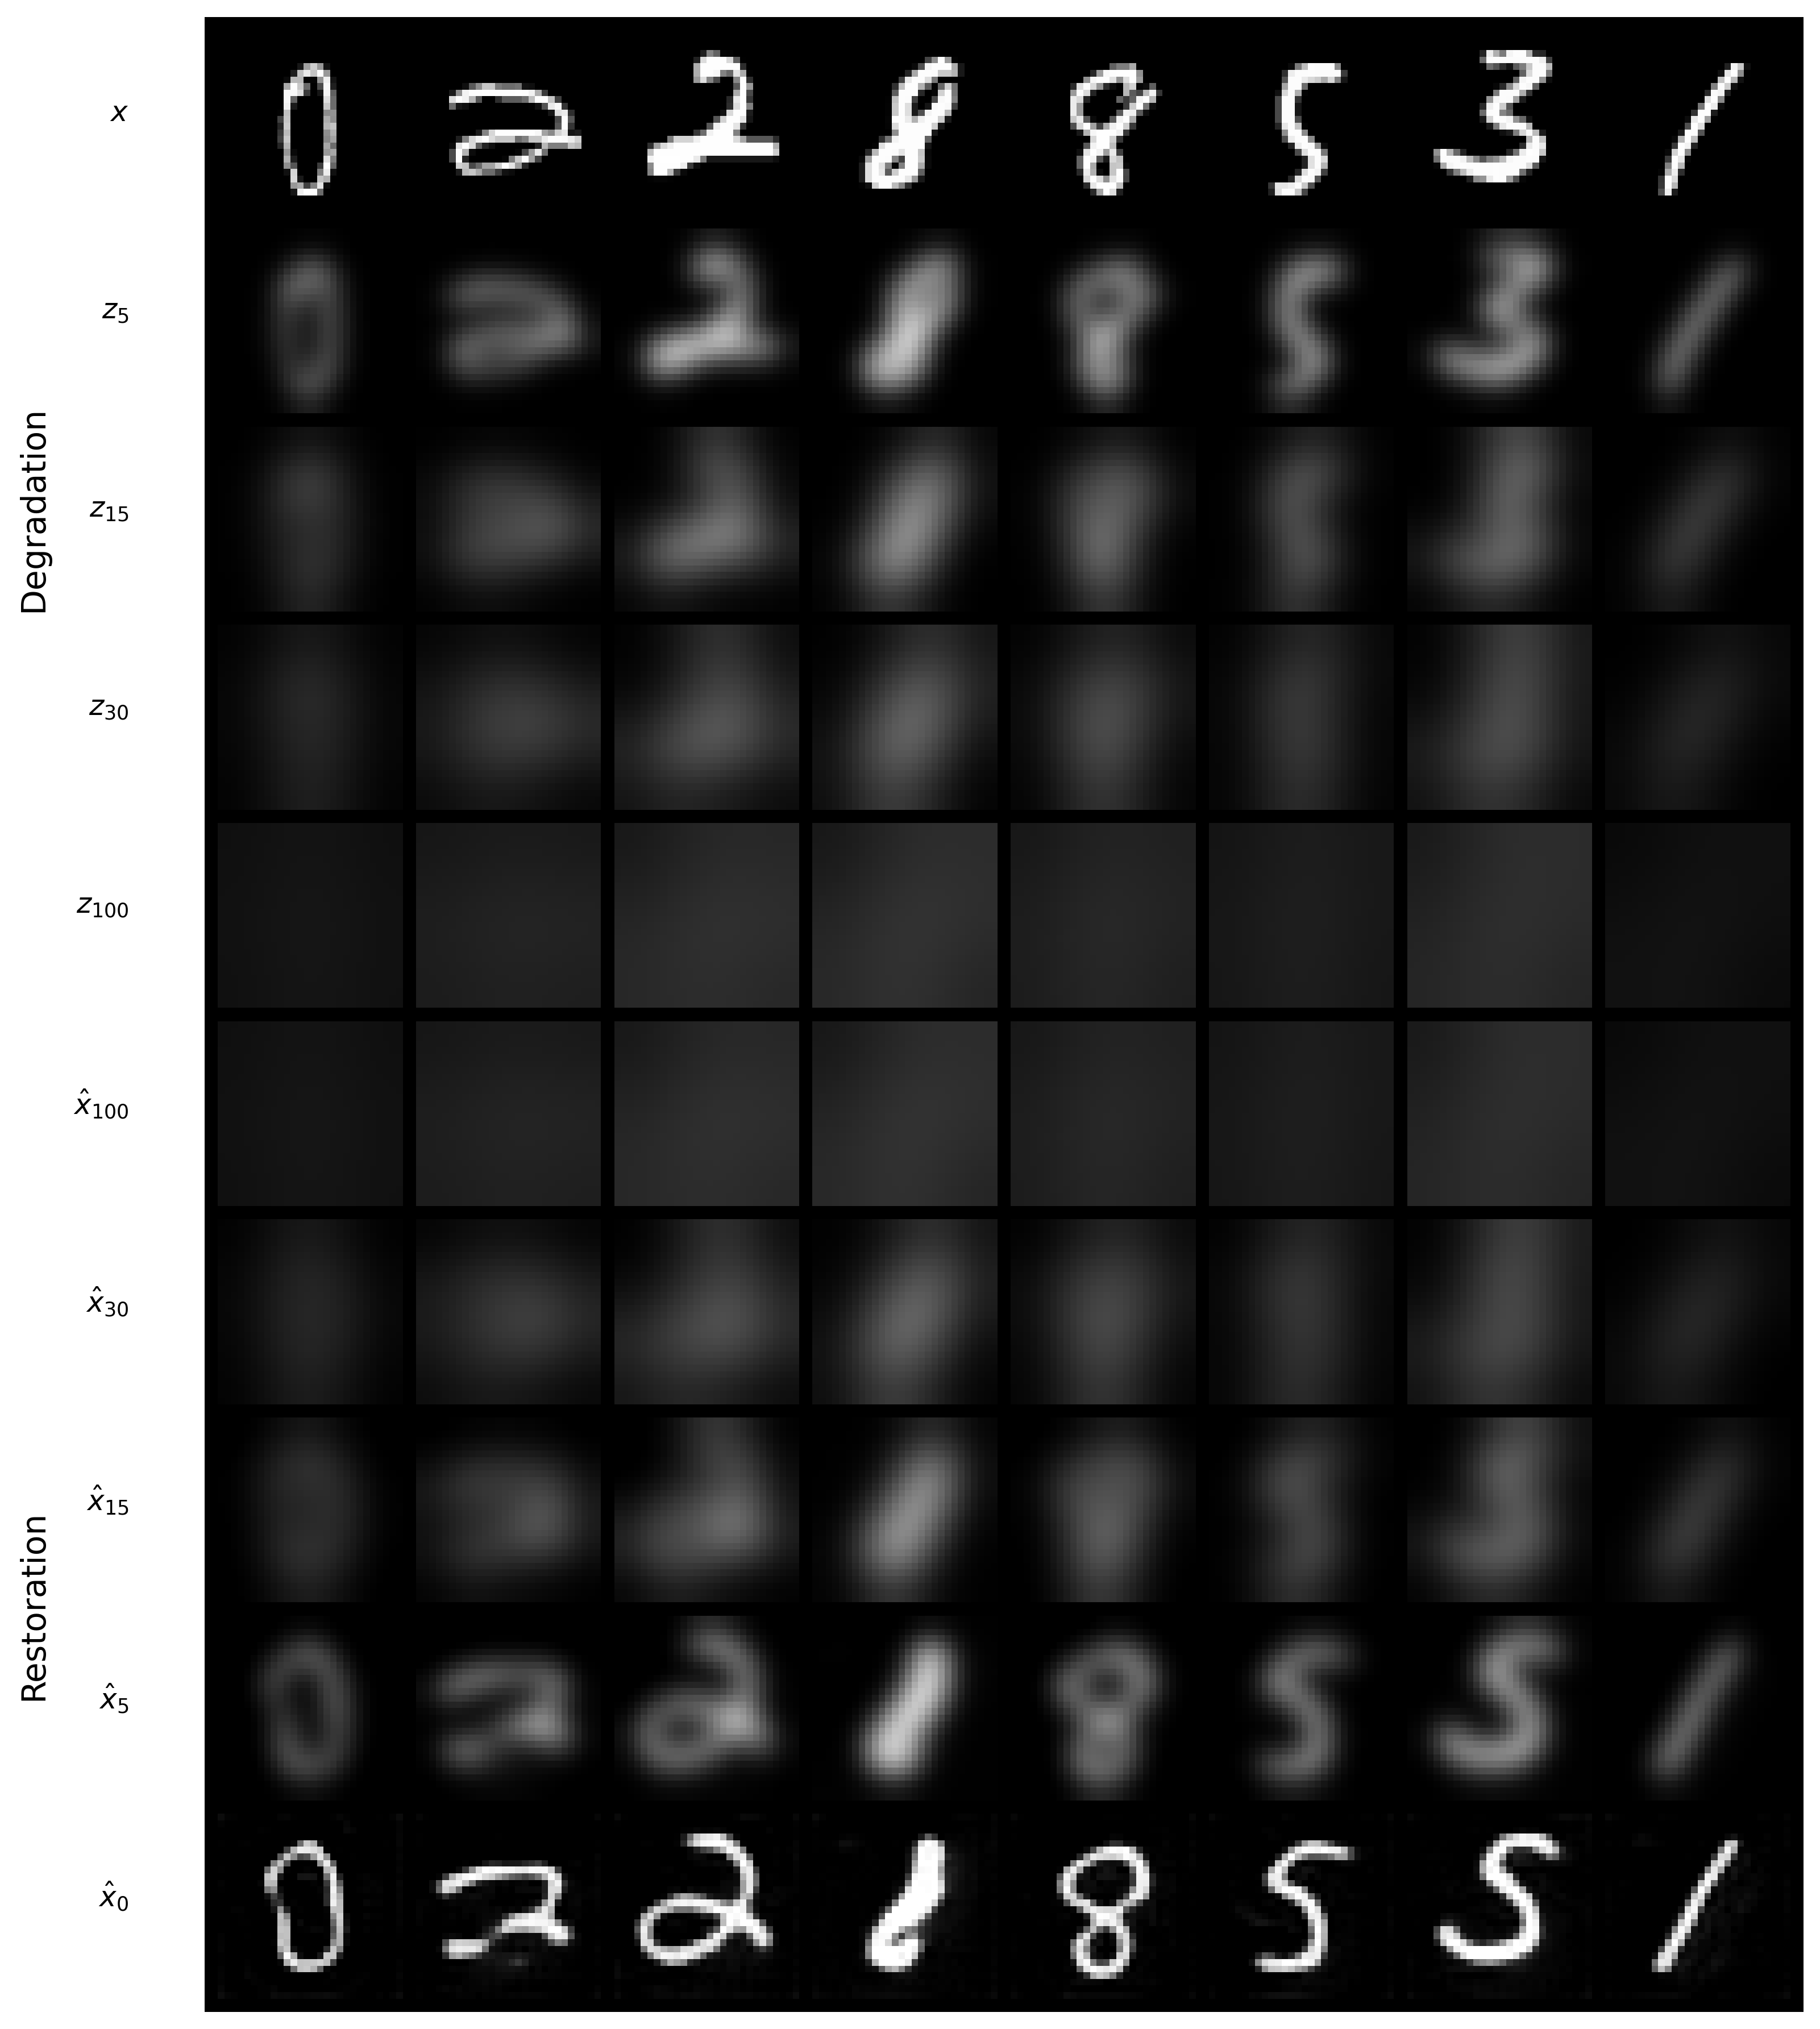
\includegraphics[width=0.9\linewidth]{figs/q2c_blur_cond_samples_norm_8.png}
        \caption{Gaussian blur model.}
        \label{fig:cond_blur}
    \end{subfigure}
    \caption{Conditionally generated samples comparison.}
    \label{fig:q2c_conditional_samples}
\end{figure}

\begin{figure}[H]
    \centering
    \begin{subfigure}{.4\textwidth}
        \centering
        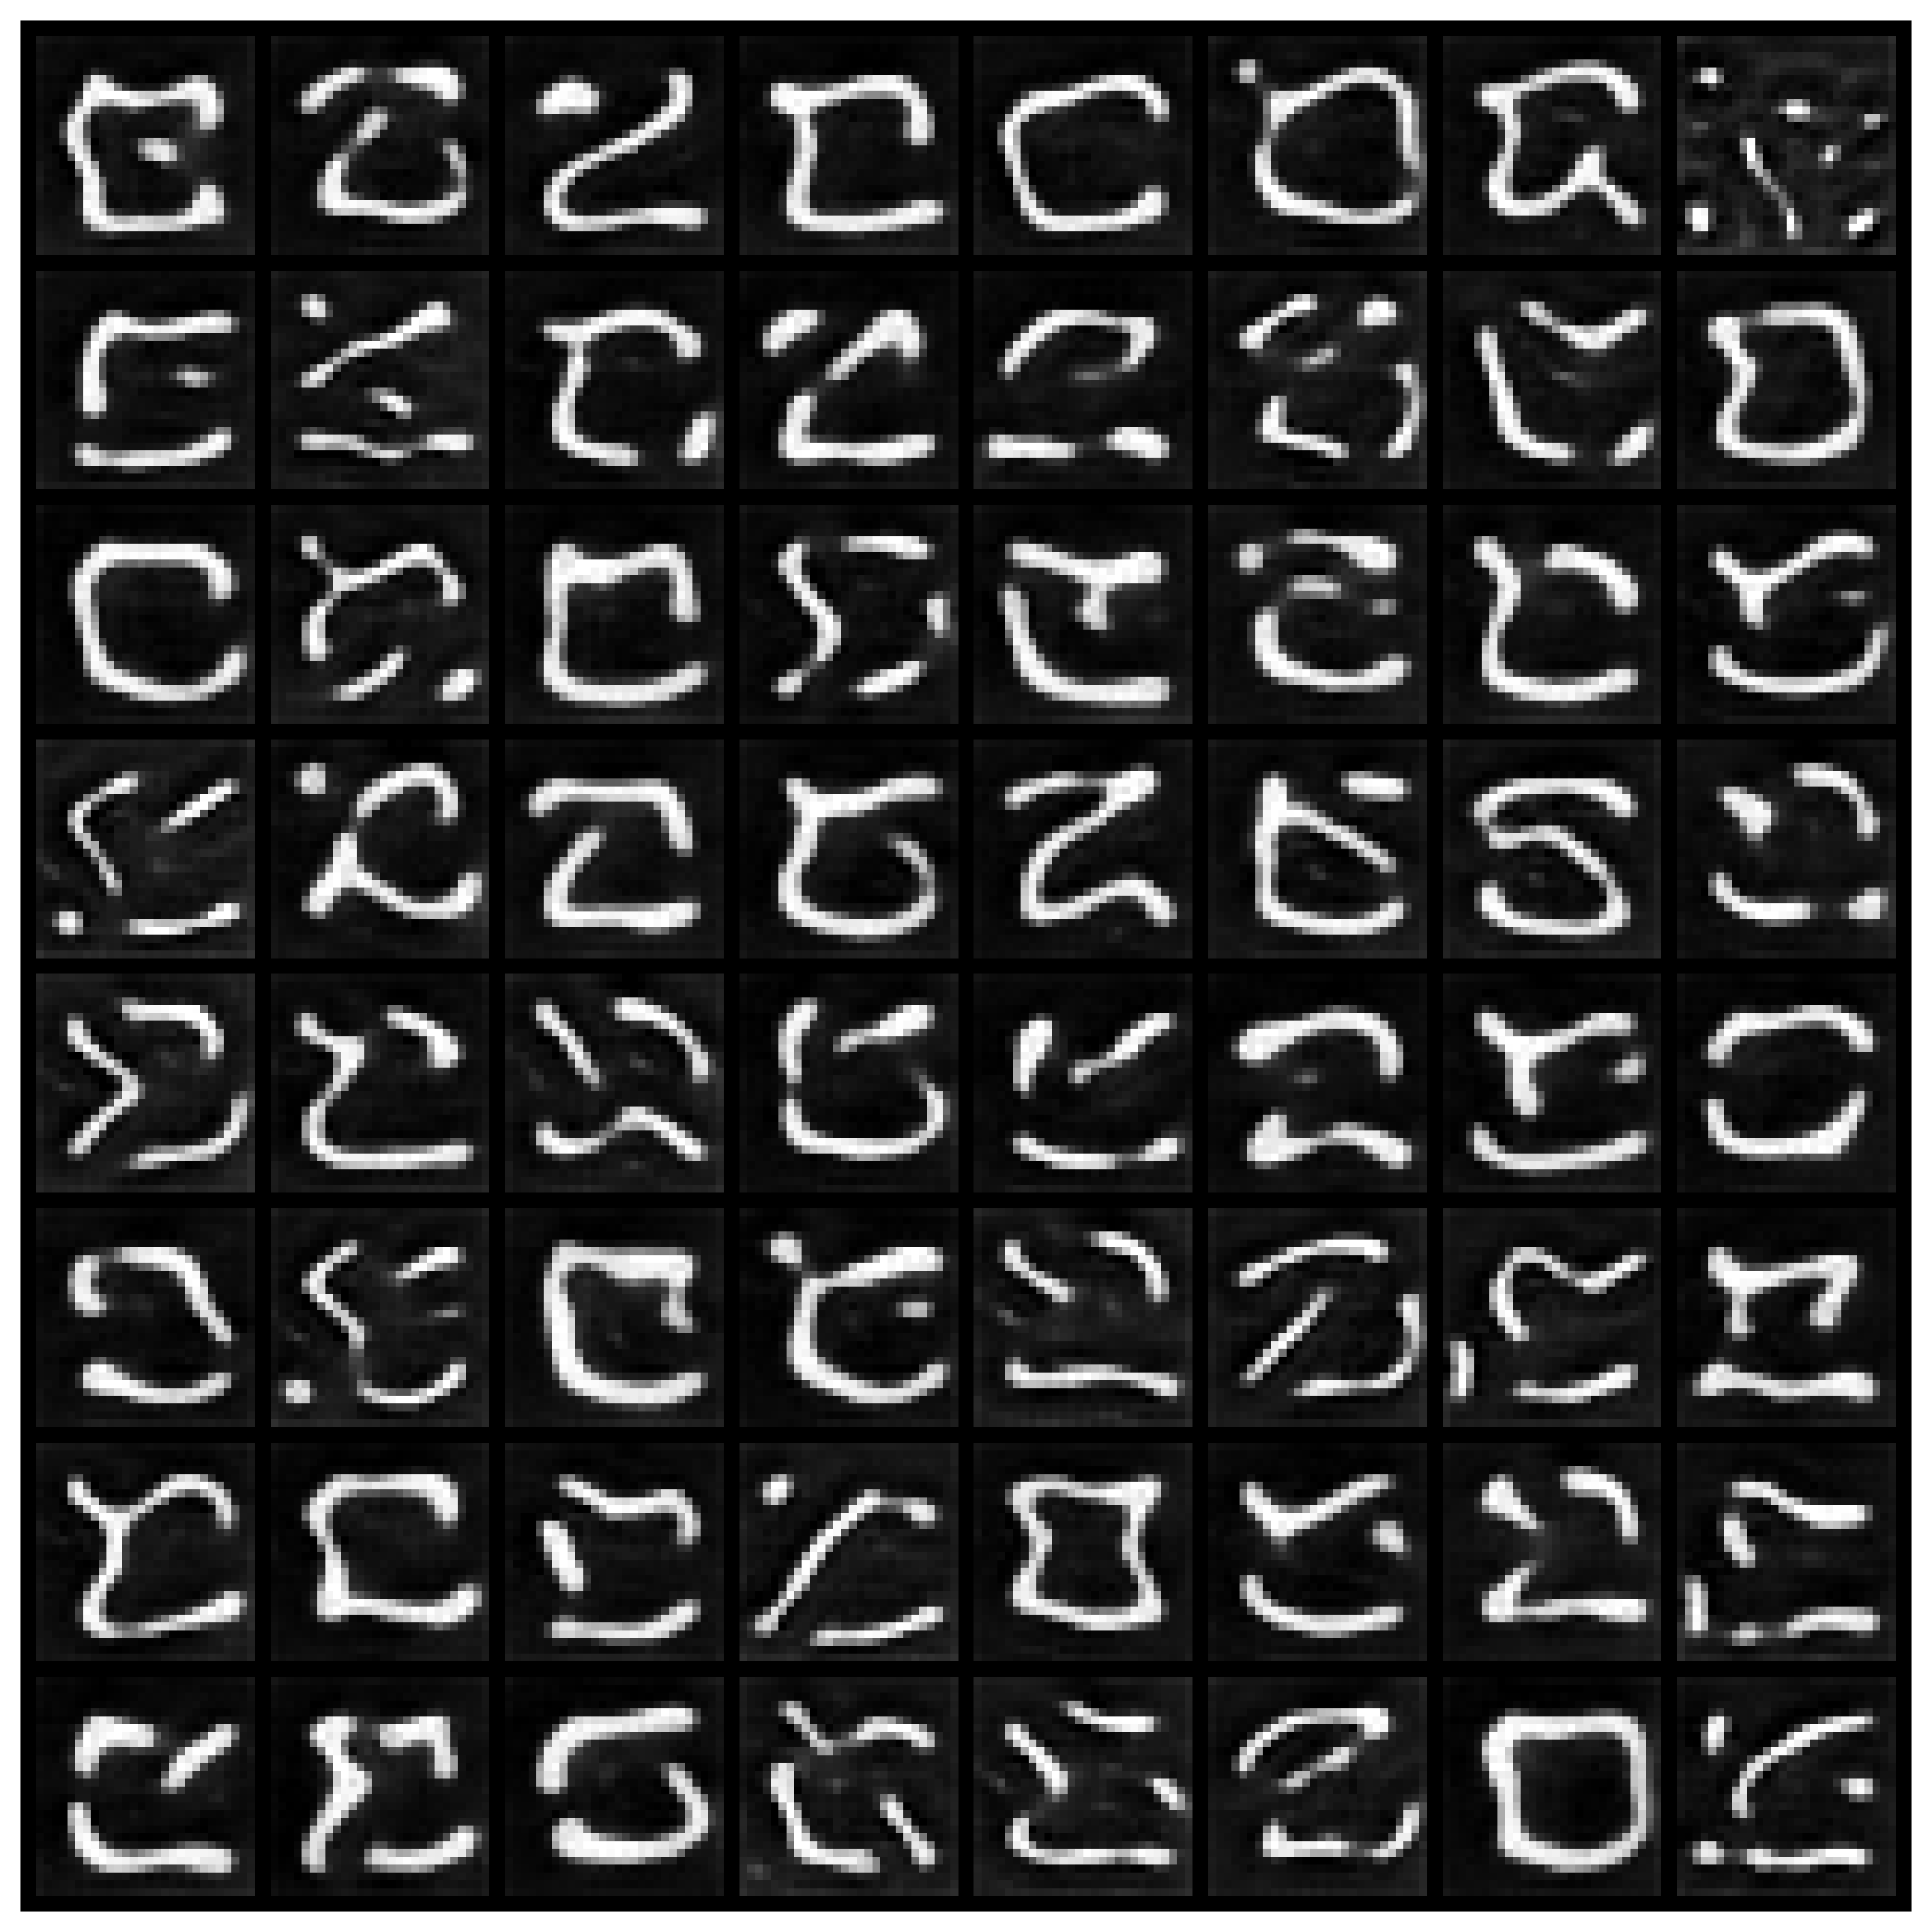
\includegraphics[width=0.9\linewidth]{figs/q2c_blur_uncond_samples_64.png}
        \caption{Gaussian blur model.}
        \label{fig:uncond_blur}
    \end{subfigure}%
    \hfill
    \begin{subfigure}{.4\textwidth}
        \centering
        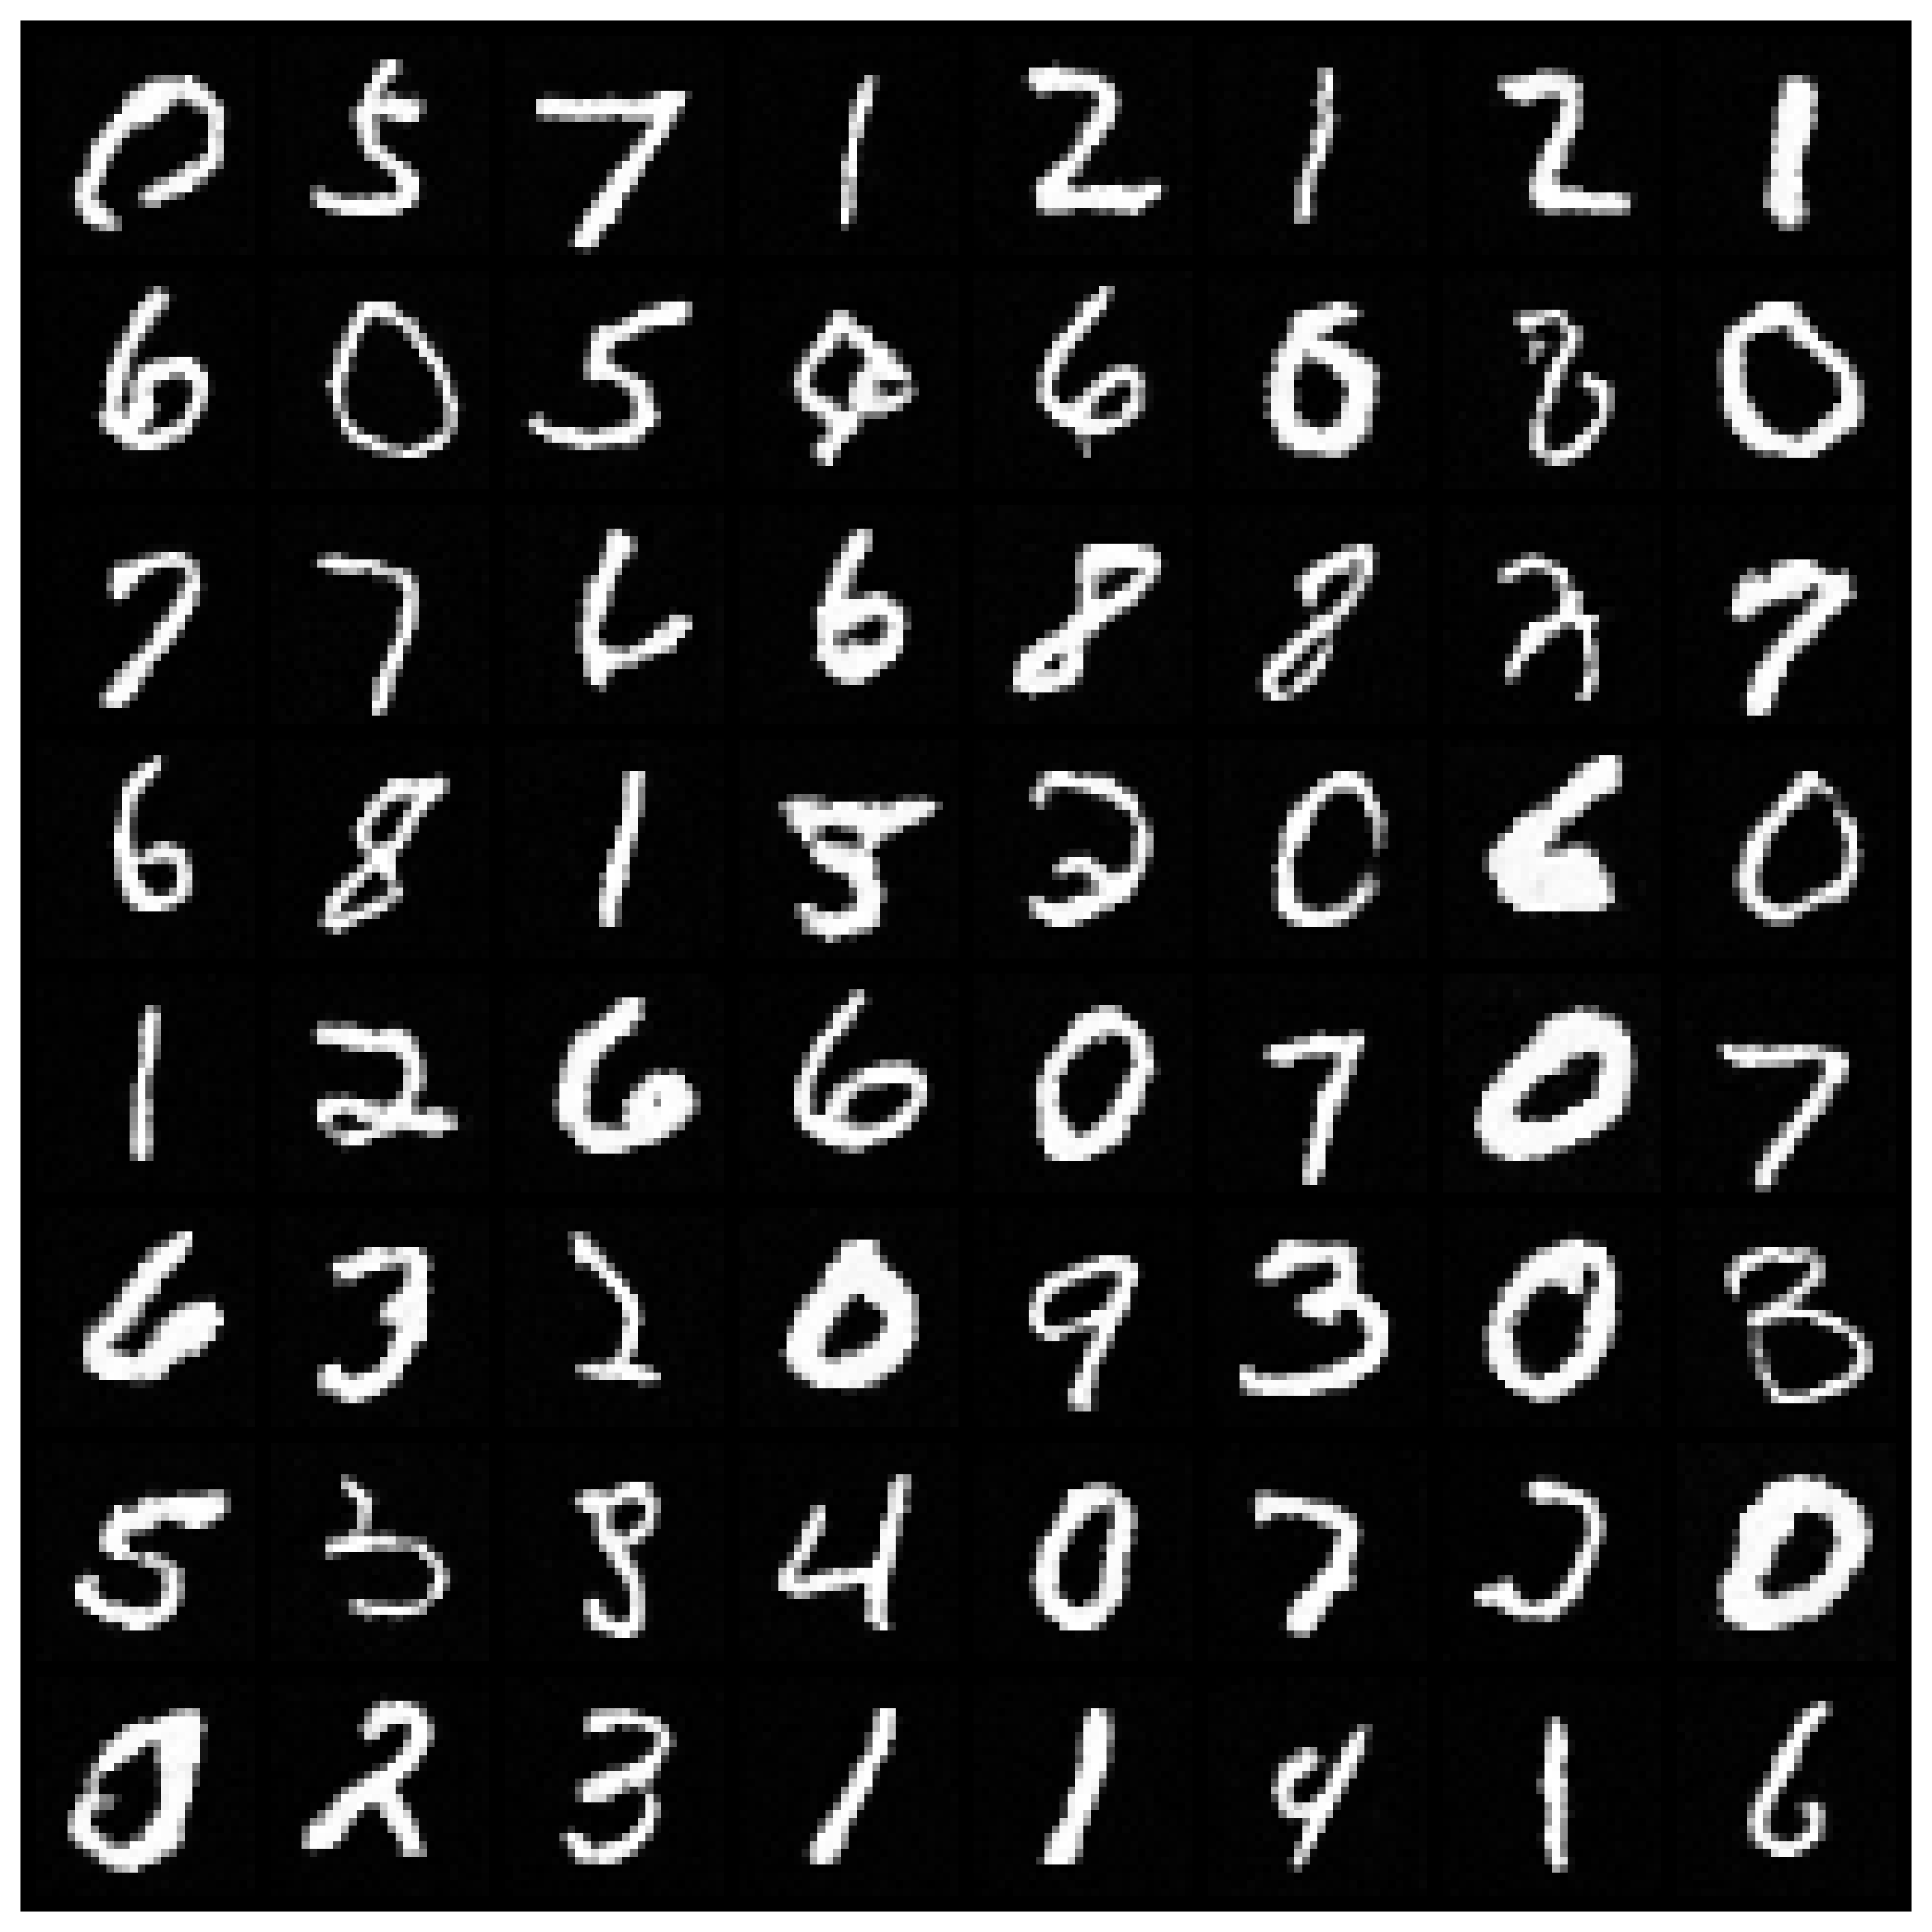
\includegraphics[width=0.9\linewidth]{figs/q2c_ddpm_uncond_samples_64.png}
        \caption{Gaussian noise model.}
        \label{fig:uncond_ddpm}
    \end{subfigure}
    \caption{Unconditionally generated samples comparison.}
    \label{fig:q2c_unconditional_samples}
\end{figure}
The quality of the conditionally generated samples shown in figure \ref{fig:q2c_conditional_samples} are quite good for both models. It is interesting to note that in 7/8 cases, the Gaussian blur models conditional reconstructions were of the same class of digit as the original. This is not the case for the Gaussian noise model which is able to reconstruct a digit with high fidelity but in most cases, a digit that belongs to a different class. Further investigation is needed to see if this result holds when blurring for more time steps.
\section{Future work}
Future work would include trying to build different representations for the latent space of the Gaussian blur model to improve it's unconditional generation capabilities. The Gaussian blur model could also be run for a larger number of steps to see if the latent space then becomes better described by the uniform image. This would also help test if the conditionally generated samples are able to as easily reconstruct the original image.

\bibliographystyle{plain}
\bibliography{ref.bib}

\section{Appendix}
\subsection{CoPilot and ChatGPT usage}
GitHub CoPilot was used heavily to to generate the code in \texttt{src/figs.ipynb}. It was also used to create the docstrings for the functions and classes in this repository. CoPilot was also used to help define and format the figures and tables in this report. ChatGPT was used to help define the functions \texttt{normalise\_batch}, \texttt{generate\_gradient\_image\_gray\_angle} and \texttt{generate\_batch\_gradient\_images} in the \texttt{src/utils.py} script, however these functions were not used in the final script and have been commented out.
\end{document}
